
\chapter{Housing Prices Appendix}

\begin{figure*}[h!]
  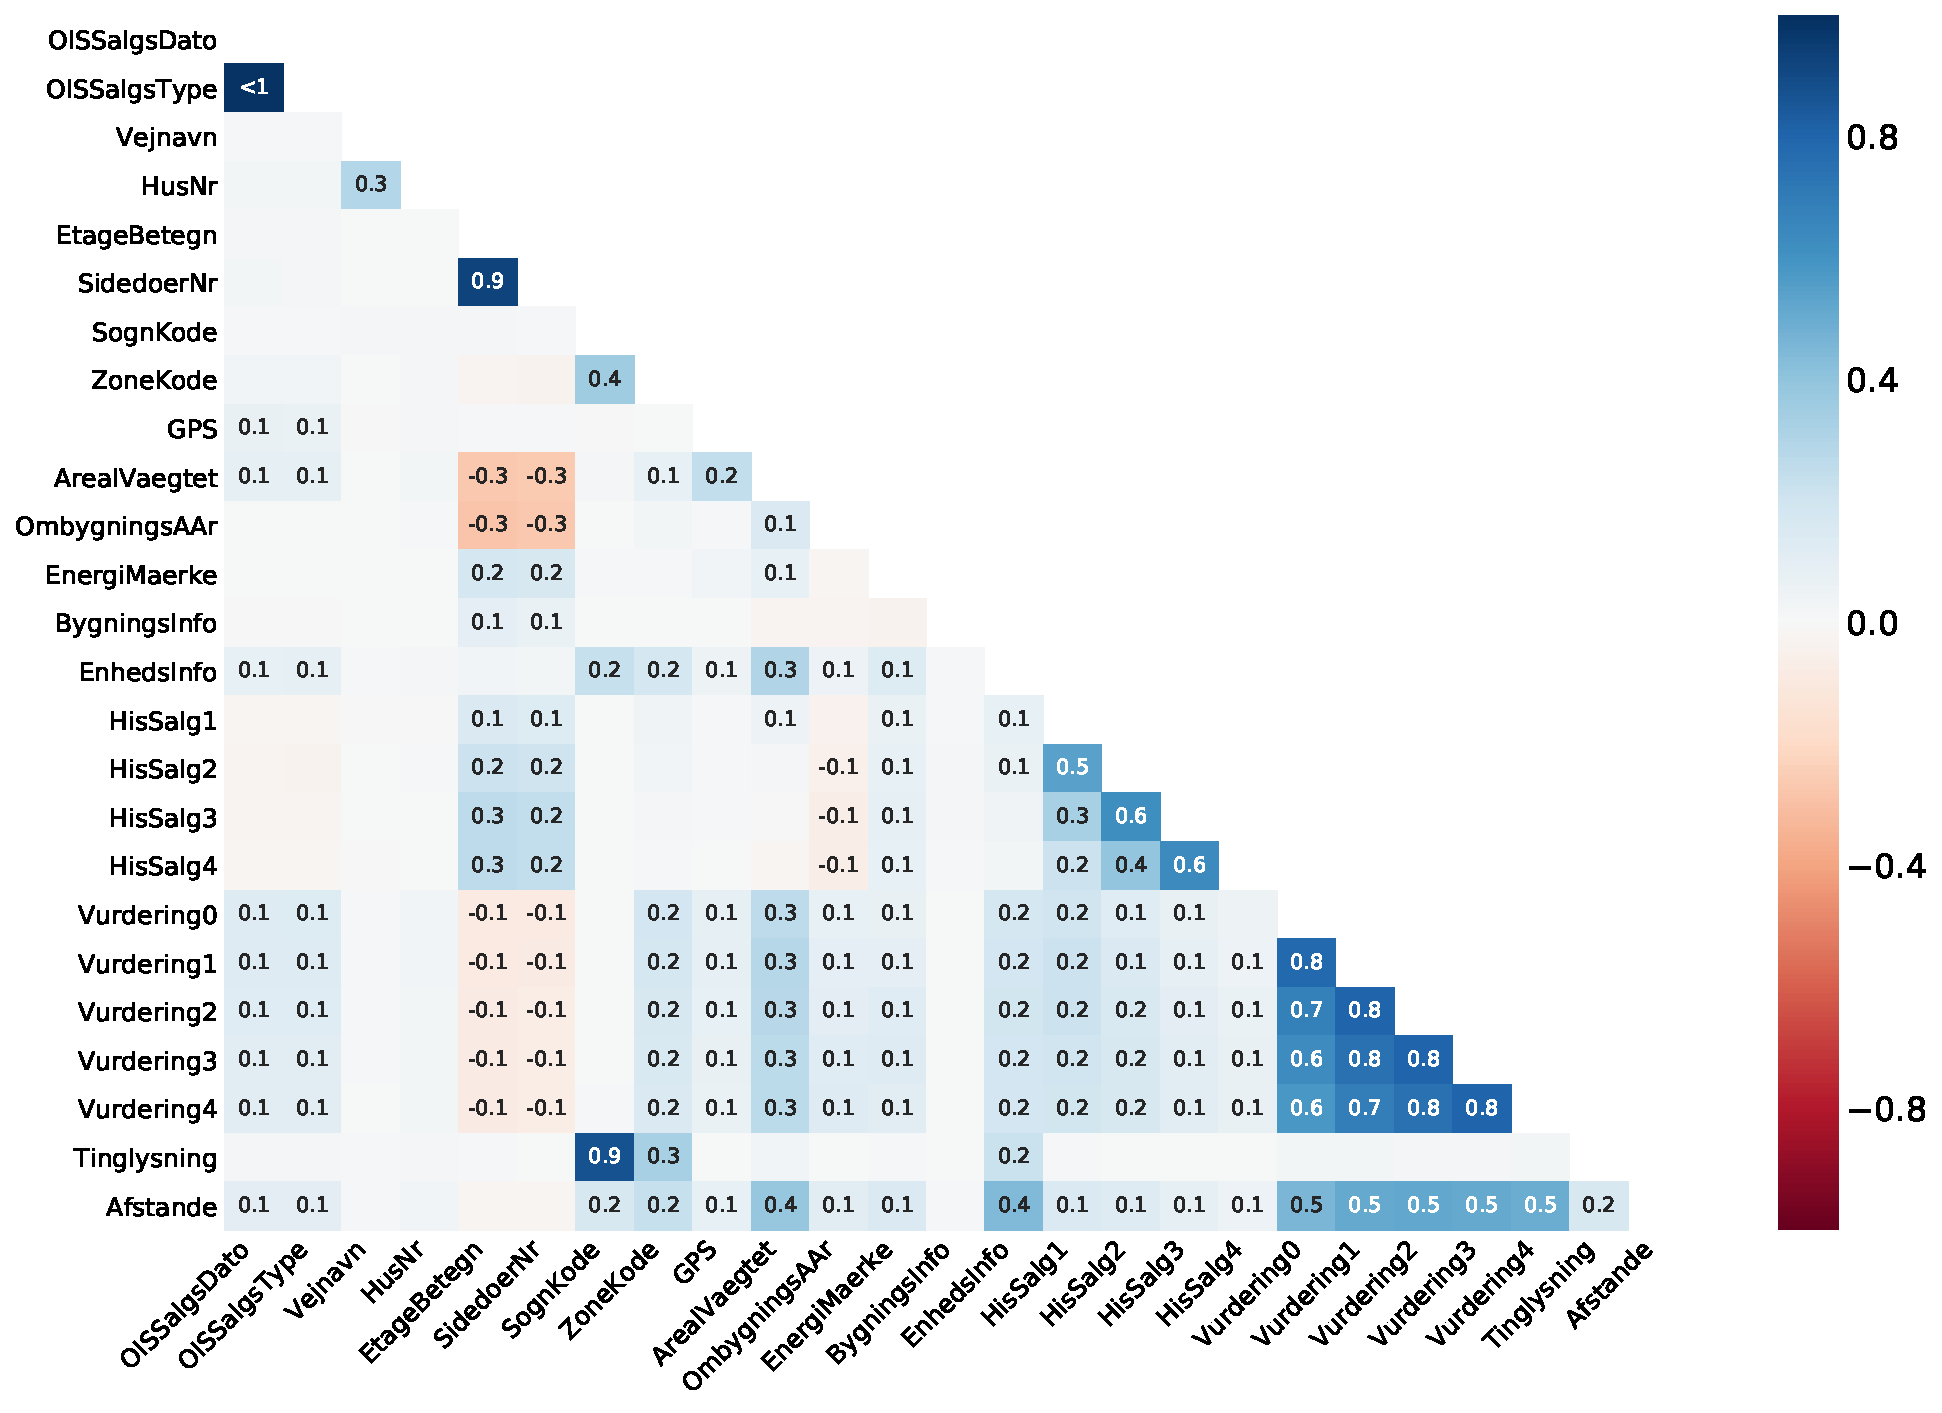
\includegraphics[draft, width=0.9\textwidth, trim=10 10 10 10, clip]{figures/housing/missing_heatmap.pdf}
  \caption[Validity Heatmap]
          {XXXX \TODO.}
  \label{fig:h:nans_heatmap}
\end{figure*}


% Input all 1D-variables for housing
% \begin{figure*}
  \centering
  \subfloat{\qquad}
  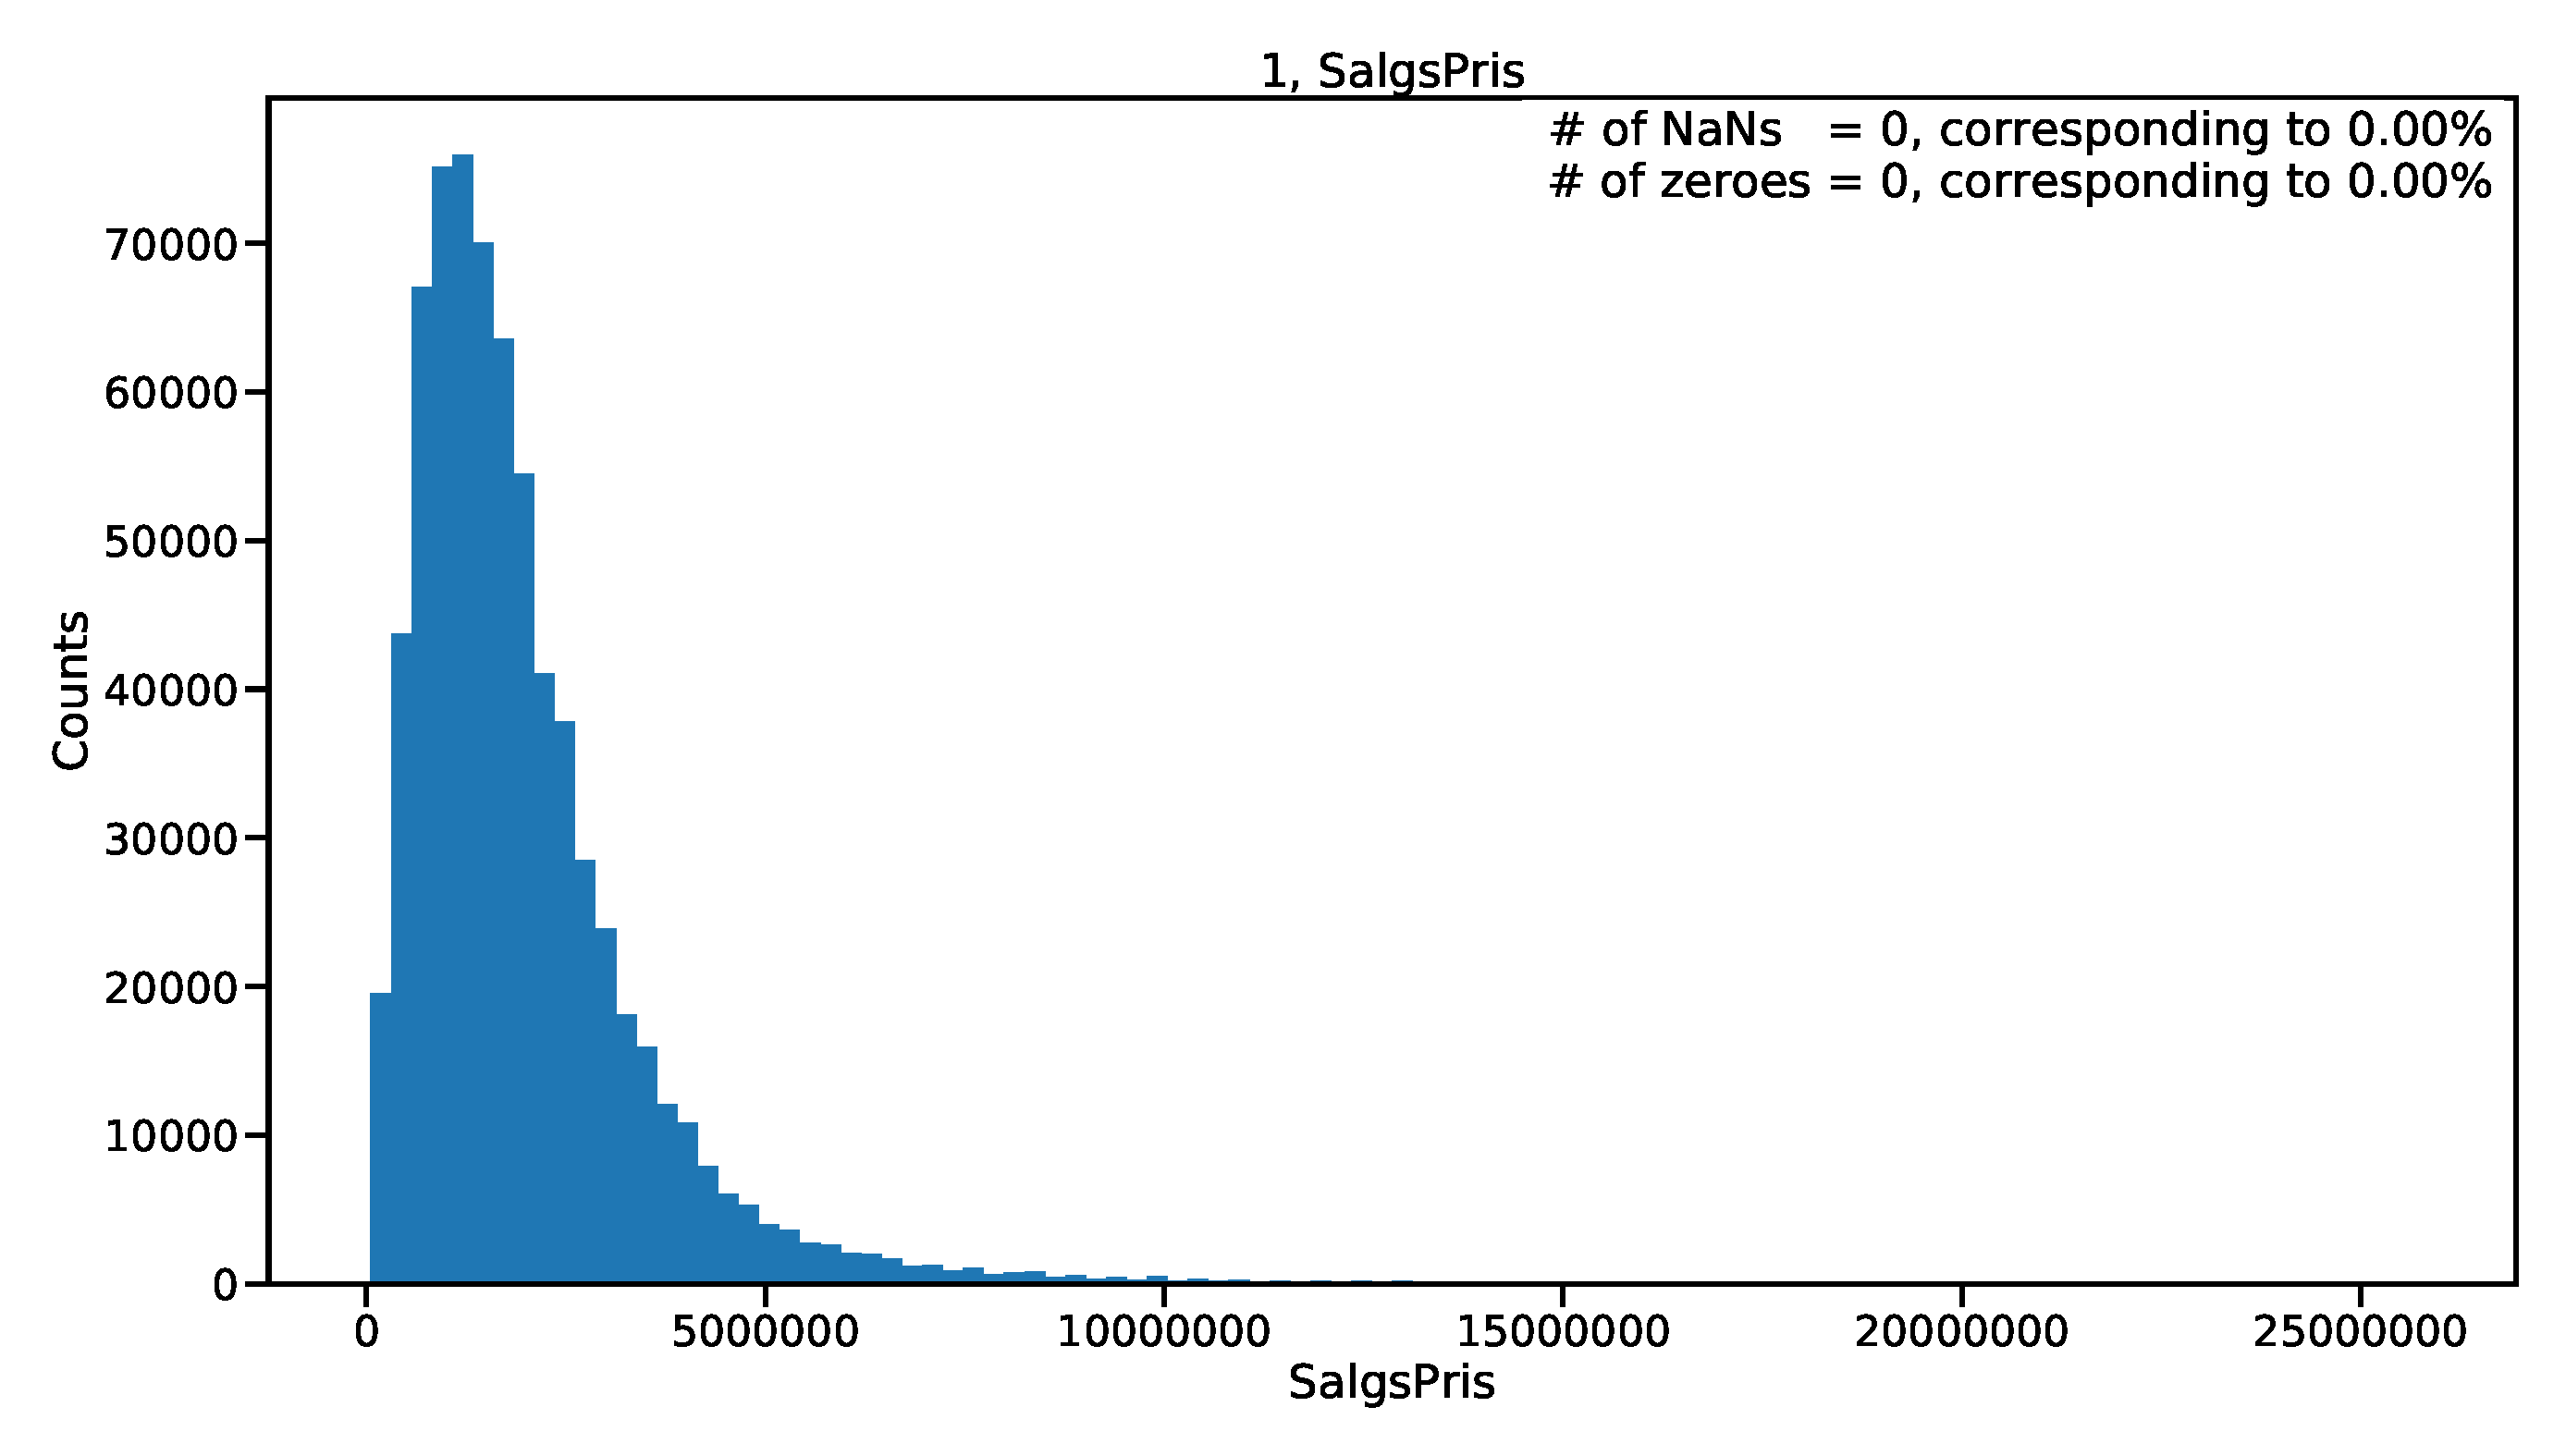
\includegraphics[width=0.45\textwidth, page=1, trim=15 0 15 0, clip]{figures/housing/overview_fig.pdf}\hfil
  \subfloat{\qquad}
  \includegraphics[width=0.45\textwidth, page=2, trim=15 0 15 0, clip]{figures/housing/overview_fig.pdf}
  \subfloat{\qquad}
  \includegraphics[width=0.45\textwidth, page=3, trim=15 0 15 0, clip]{figures/housing/overview_fig.pdf}\hfil
  \subfloat{\qquad}
  \includegraphics[width=0.45\textwidth, page=4, trim=15 0 15 0, clip]{figures/housing/overview_fig.pdf}
  \subfloat{\qquad}
  \includegraphics[width=0.45\textwidth, page=5, trim=15 0 15 0, clip]{figures/housing/overview_fig.pdf}\hfil
  \subfloat{\qquad}
  \includegraphics[width=0.45\textwidth, page=6, trim=15 0 15 0, clip]{figures/housing/overview_fig.pdf}
  \subfloat{\qquad}
  \includegraphics[width=0.45\textwidth, page=7, trim=15 0 15 0, clip]{figures/housing/overview_fig.pdf}\hfil
  \subfloat{\qquad}
  \includegraphics[width=0.45\textwidth, page=8, trim=15 0 15 0, clip]{figures/housing/overview_fig.pdf}
  \subfloat{\qquad}
  \includegraphics[width=0.45\textwidth, page=9, trim=15 0 15 0, clip]{figures/housing/overview_fig.pdf}\hfil
  \subfloat{\qquad}
  \includegraphics[width=0.45\textwidth, page=10, trim=15 0 15 0, clip]{figures/housing/overview_fig.pdf}
  \subfloat{\qquad}
  \includegraphics[width=0.45\textwidth, page=11, trim=15 0 15 0, clip]{figures/housing/overview_fig.pdf}\hfil
  \subfloat{\qquad}
  \includegraphics[width=0.45\textwidth, page=12, trim=15 0 15 0, clip]{figures/housing/overview_fig.pdf}
  \caption[Distributions for the housing price dataset]{Distributions the 168 input variables (excluding \code{ID} and \code{Vejnavn}).}
  \label{fig:h:variable_overview_all_1}
  \vspace{\abovecaptionskip}
\end{figure*}

\begin{figure*}
  \centering
  \subfloat{\qquad}
  \includegraphics[width=0.45\textwidth, page=13, trim=15 0 15 0, clip]{figures/housing/overview_fig.pdf}\hfil
  \subfloat{\qquad}
  \includegraphics[width=0.45\textwidth, page=14, trim=15 0 15 0, clip]{figures/housing/overview_fig.pdf}
  \subfloat{\qquad}
  \includegraphics[width=0.45\textwidth, page=15, trim=15 0 15 0, clip]{figures/housing/overview_fig.pdf}\hfil
  \subfloat{\qquad}
  \includegraphics[width=0.45\textwidth, page=16, trim=15 0 15 0, clip]{figures/housing/overview_fig.pdf}
  \subfloat{\qquad}
  \includegraphics[width=0.45\textwidth, page=17, trim=15 0 15 0, clip]{figures/housing/overview_fig.pdf}\hfil
  \subfloat{\qquad}
  \includegraphics[width=0.45\textwidth, page=18, trim=15 0 15 0, clip]{figures/housing/overview_fig.pdf}
  \subfloat{\qquad}
  \includegraphics[width=0.45\textwidth, page=19, trim=15 0 15 0, clip]{figures/housing/overview_fig.pdf}\hfil
  \subfloat{\qquad}
  \includegraphics[width=0.45\textwidth, page=20, trim=15 0 15 0, clip]{figures/housing/overview_fig.pdf}
  \subfloat{\qquad}
  \includegraphics[width=0.45\textwidth, page=21, trim=15 0 15 0, clip]{figures/housing/overview_fig.pdf}\hfil
  \subfloat{\qquad}
  \includegraphics[width=0.45\textwidth, page=22, trim=15 0 15 0, clip]{figures/housing/overview_fig.pdf}
  \subfloat{\qquad}
  \includegraphics[width=0.45\textwidth, page=23, trim=15 0 15 0, clip]{figures/housing/overview_fig.pdf}\hfil
  \subfloat{\qquad}
  \includegraphics[width=0.45\textwidth, page=24, trim=15 0 15 0, clip]{figures/housing/overview_fig.pdf}
  \caption[Distributions for the housing price dataset]{Distributions the 168 input variables (excluding \code{ID} and \code{Vejnavn}).}
  \label{fig:h:variable_overview_all_2}
  \vspace{\abovecaptionskip}
\end{figure*}

\begin{figure*}
  \centering
  \subfloat{\qquad}
  \includegraphics[width=0.45\textwidth, page=25, trim=15 0 15 0, clip]{figures/housing/overview_fig.pdf}\hfil
  \subfloat{\qquad}
  \includegraphics[width=0.45\textwidth, page=26, trim=15 0 15 0, clip]{figures/housing/overview_fig.pdf}
  \subfloat{\qquad}
  \includegraphics[width=0.45\textwidth, page=27, trim=15 0 15 0, clip]{figures/housing/overview_fig.pdf}\hfil
  \subfloat{\qquad}
  \includegraphics[width=0.45\textwidth, page=28, trim=15 0 15 0, clip]{figures/housing/overview_fig.pdf}
  \subfloat{\qquad}
  \includegraphics[width=0.45\textwidth, page=29, trim=15 0 15 0, clip]{figures/housing/overview_fig.pdf}\hfil
  \subfloat{\qquad}
  \includegraphics[width=0.45\textwidth, page=30, trim=15 0 15 0, clip]{figures/housing/overview_fig.pdf}
  \subfloat{\qquad}
  \includegraphics[width=0.45\textwidth, page=31, trim=15 0 15 0, clip]{figures/housing/overview_fig.pdf}\hfil
  \subfloat{\qquad}
  \includegraphics[width=0.45\textwidth, page=32, trim=15 0 15 0, clip]{figures/housing/overview_fig.pdf}
  \subfloat{\qquad}
  \includegraphics[width=0.45\textwidth, page=33, trim=15 0 15 0, clip]{figures/housing/overview_fig.pdf}\hfil
  \subfloat{\qquad}
  \includegraphics[width=0.45\textwidth, page=34, trim=15 0 15 0, clip]{figures/housing/overview_fig.pdf}
  \subfloat{\qquad}
  \includegraphics[width=0.45\textwidth, page=35, trim=15 0 15 0, clip]{figures/housing/overview_fig.pdf}\hfil
  \subfloat{\qquad}
  \includegraphics[width=0.45\textwidth, page=36, trim=15 0 15 0, clip]{figures/housing/overview_fig.pdf}
  \caption[Distributions for the housing price dataset]{Distributions the 168 input variables (excluding \code{ID} and \code{Vejnavn}).}
  \label{fig:h:variable_overview_all_3}
  \vspace{\abovecaptionskip}
\end{figure*}

\begin{figure*}
  \centering
  \subfloat{\qquad}
  \includegraphics[width=0.45\textwidth, page=37, trim=15 0 15 0, clip]{figures/housing/overview_fig.pdf}\hfil
  \subfloat{\qquad}
  \includegraphics[width=0.45\textwidth, page=38, trim=15 0 15 0, clip]{figures/housing/overview_fig.pdf}
  \subfloat{\qquad}
  \includegraphics[width=0.45\textwidth, page=39, trim=15 0 15 0, clip]{figures/housing/overview_fig.pdf}\hfil
  \subfloat{\qquad}
  \includegraphics[width=0.45\textwidth, page=40, trim=15 0 15 0, clip]{figures/housing/overview_fig.pdf}
  \subfloat{\qquad}
  \includegraphics[width=0.45\textwidth, page=41, trim=15 0 15 0, clip]{figures/housing/overview_fig.pdf}\hfil
  \subfloat{\qquad}
  \includegraphics[width=0.45\textwidth, page=42, trim=15 0 15 0, clip]{figures/housing/overview_fig.pdf}
  \subfloat{\qquad}
  \includegraphics[width=0.45\textwidth, page=43, trim=15 0 15 0, clip]{figures/housing/overview_fig.pdf}\hfil
  \subfloat{\qquad}
  \includegraphics[width=0.45\textwidth, page=44, trim=15 0 15 0, clip]{figures/housing/overview_fig.pdf}
  \subfloat{\qquad}
  \includegraphics[width=0.45\textwidth, page=45, trim=15 0 15 0, clip]{figures/housing/overview_fig.pdf}\hfil
  \subfloat{\qquad}
  \includegraphics[width=0.45\textwidth, page=46, trim=15 0 15 0, clip]{figures/housing/overview_fig.pdf}
  \subfloat{\qquad}
  \includegraphics[width=0.45\textwidth, page=47, trim=15 0 15 0, clip]{figures/housing/overview_fig.pdf}\hfil
  \subfloat{\qquad}
  \includegraphics[width=0.45\textwidth, page=48, trim=15 0 15 0, clip]{figures/housing/overview_fig.pdf}
  \caption[Distributions for the housing price dataset]{Distributions the 168 input variables (excluding \code{ID} and \code{Vejnavn}).}
  \label{fig:h:variable_overview_all_4}
  \vspace{\abovecaptionskip}
\end{figure*}

\begin{figure*}
  \centering
  \subfloat{\qquad}
  \includegraphics[width=0.45\textwidth, page=49, trim=15 0 15 0, clip]{figures/housing/overview_fig.pdf}\hfil
  \subfloat{\qquad}
  \includegraphics[width=0.45\textwidth, page=50, trim=15 0 15 0, clip]{figures/housing/overview_fig.pdf}
  \subfloat{\qquad}
  \includegraphics[width=0.45\textwidth, page=51, trim=15 0 15 0, clip]{figures/housing/overview_fig.pdf}\hfil
  \subfloat{\qquad}
  \includegraphics[width=0.45\textwidth, page=52, trim=15 0 15 0, clip]{figures/housing/overview_fig.pdf}
  \subfloat{\qquad}
  \includegraphics[width=0.45\textwidth, page=53, trim=15 0 15 0, clip]{figures/housing/overview_fig.pdf}\hfil
  \subfloat{\qquad}
  \includegraphics[width=0.45\textwidth, page=54, trim=15 0 15 0, clip]{figures/housing/overview_fig.pdf}
  \subfloat{\qquad}
  \includegraphics[width=0.45\textwidth, page=55, trim=15 0 15 0, clip]{figures/housing/overview_fig.pdf}\hfil
  \subfloat{\qquad}
  \includegraphics[width=0.45\textwidth, page=56, trim=15 0 15 0, clip]{figures/housing/overview_fig.pdf}
  \subfloat{\qquad}
  \includegraphics[width=0.45\textwidth, page=57, trim=15 0 15 0, clip]{figures/housing/overview_fig.pdf}\hfil
  \subfloat{\qquad}
  \includegraphics[width=0.45\textwidth, page=58, trim=15 0 15 0, clip]{figures/housing/overview_fig.pdf}
  \subfloat{\qquad}
  \includegraphics[width=0.45\textwidth, page=59, trim=15 0 15 0, clip]{figures/housing/overview_fig.pdf}\hfil
  \subfloat{\qquad}
  \includegraphics[width=0.45\textwidth, page=60, trim=15 0 15 0, clip]{figures/housing/overview_fig.pdf}
  \caption[Distributions for the housing price dataset]{Distributions the 168 input variables (excluding \code{ID} and \code{Vejnavn}).}
  \label{fig:h:variable_overview_all_5}
  \vspace{\abovecaptionskip}
\end{figure*}

\begin{figure*}
  \centering
  \subfloat{\qquad}
  \includegraphics[width=0.45\textwidth, page=61, trim=15 0 15 0, clip]{figures/housing/overview_fig.pdf}\hfil
  \subfloat{\qquad}
  \includegraphics[width=0.45\textwidth, page=62, trim=15 0 15 0, clip]{figures/housing/overview_fig.pdf}
  \subfloat{\qquad}
  \includegraphics[width=0.45\textwidth, page=63, trim=15 0 15 0, clip]{figures/housing/overview_fig.pdf}\hfil
  \subfloat{\qquad}
  \includegraphics[width=0.45\textwidth, page=64, trim=15 0 15 0, clip]{figures/housing/overview_fig.pdf}
  \subfloat{\qquad}
  \includegraphics[width=0.45\textwidth, page=65, trim=15 0 15 0, clip]{figures/housing/overview_fig.pdf}\hfil
  \subfloat{\qquad}
  \includegraphics[width=0.45\textwidth, page=66, trim=15 0 15 0, clip]{figures/housing/overview_fig.pdf}
  \subfloat{\qquad}
  \includegraphics[width=0.45\textwidth, page=67, trim=15 0 15 0, clip]{figures/housing/overview_fig.pdf}\hfil
  \subfloat{\qquad}
  \includegraphics[width=0.45\textwidth, page=68, trim=15 0 15 0, clip]{figures/housing/overview_fig.pdf}
  \subfloat{\qquad}
  \includegraphics[width=0.45\textwidth, page=69, trim=15 0 15 0, clip]{figures/housing/overview_fig.pdf}\hfil
  \subfloat{\qquad}
  \includegraphics[width=0.45\textwidth, page=70, trim=15 0 15 0, clip]{figures/housing/overview_fig.pdf}
  \subfloat{\qquad}
  \includegraphics[width=0.45\textwidth, page=71, trim=15 0 15 0, clip]{figures/housing/overview_fig.pdf}\hfil
  \subfloat{\qquad}
  \includegraphics[width=0.45\textwidth, page=72, trim=15 0 15 0, clip]{figures/housing/overview_fig.pdf}
  \caption[Distributions for the housing price dataset]{Distributions the 168 input variables (excluding \code{ID} and \code{Vejnavn}).}
  \label{fig:h:variable_overview_all_6}
  \vspace{\abovecaptionskip}
\end{figure*}

\begin{figure*}
  \centering
  \subfloat{\qquad}
  \includegraphics[width=0.45\textwidth, page=73, trim=15 0 15 0, clip]{figures/housing/overview_fig.pdf}\hfil
  \subfloat{\qquad}
  \includegraphics[width=0.45\textwidth, page=74, trim=15 0 15 0, clip]{figures/housing/overview_fig.pdf}
  \subfloat{\qquad}
  \includegraphics[width=0.45\textwidth, page=75, trim=15 0 15 0, clip]{figures/housing/overview_fig.pdf}\hfil
  \subfloat{\qquad}
  \includegraphics[width=0.45\textwidth, page=76, trim=15 0 15 0, clip]{figures/housing/overview_fig.pdf}
  \subfloat{\qquad}
  \includegraphics[width=0.45\textwidth, page=77, trim=15 0 15 0, clip]{figures/housing/overview_fig.pdf}\hfil
  \subfloat{\qquad}
  \includegraphics[width=0.45\textwidth, page=78, trim=15 0 15 0, clip]{figures/housing/overview_fig.pdf}
  \subfloat{\qquad}
  \includegraphics[width=0.45\textwidth, page=79, trim=15 0 15 0, clip]{figures/housing/overview_fig.pdf}\hfil
  \subfloat{\qquad}
  \includegraphics[width=0.45\textwidth, page=80, trim=15 0 15 0, clip]{figures/housing/overview_fig.pdf}
  \subfloat{\qquad}
  \includegraphics[width=0.45\textwidth, page=81, trim=15 0 15 0, clip]{figures/housing/overview_fig.pdf}\hfil
  \subfloat{\qquad}
  \includegraphics[width=0.45\textwidth, page=82, trim=15 0 15 0, clip]{figures/housing/overview_fig.pdf}
  \subfloat{\qquad}
  \includegraphics[width=0.45\textwidth, page=83, trim=15 0 15 0, clip]{figures/housing/overview_fig.pdf}\hfil
  \subfloat{\qquad}
  \includegraphics[width=0.45\textwidth, page=84, trim=15 0 15 0, clip]{figures/housing/overview_fig.pdf}
  \caption[Distributions for the housing price dataset]{Distributions the 168 input variables (excluding \code{ID} and \code{Vejnavn}).}
  \label{fig:h:variable_overview_all_7}
  \vspace{\abovecaptionskip}
\end{figure*}

\begin{figure*}
  \centering
  \subfloat{\qquad}
  \includegraphics[width=0.45\textwidth, page=85, trim=15 0 15 0, clip]{figures/housing/overview_fig.pdf}\hfil
  \subfloat{\qquad}
  \includegraphics[width=0.45\textwidth, page=86, trim=15 0 15 0, clip]{figures/housing/overview_fig.pdf}
  \subfloat{\qquad}
  \includegraphics[width=0.45\textwidth, page=87, trim=15 0 15 0, clip]{figures/housing/overview_fig.pdf}\hfil
  \subfloat{\qquad}
  \includegraphics[width=0.45\textwidth, page=88, trim=15 0 15 0, clip]{figures/housing/overview_fig.pdf}
  \subfloat{\qquad}
  \includegraphics[width=0.45\textwidth, page=89, trim=15 0 15 0, clip]{figures/housing/overview_fig.pdf}\hfil
  \subfloat{\qquad}
  \includegraphics[width=0.45\textwidth, page=90, trim=15 0 15 0, clip]{figures/housing/overview_fig.pdf}
  \subfloat{\qquad}
  \includegraphics[width=0.45\textwidth, page=91, trim=15 0 15 0, clip]{figures/housing/overview_fig.pdf}\hfil
  \subfloat{\qquad}
  \includegraphics[width=0.45\textwidth, page=92, trim=15 0 15 0, clip]{figures/housing/overview_fig.pdf}
  \subfloat{\qquad}
  \includegraphics[width=0.45\textwidth, page=93, trim=15 0 15 0, clip]{figures/housing/overview_fig.pdf}\hfil
  \subfloat{\qquad}
  \includegraphics[width=0.45\textwidth, page=94, trim=15 0 15 0, clip]{figures/housing/overview_fig.pdf}
  \subfloat{\qquad}
  \includegraphics[width=0.45\textwidth, page=95, trim=15 0 15 0, clip]{figures/housing/overview_fig.pdf}\hfil
  \subfloat{\qquad}
  \includegraphics[width=0.45\textwidth, page=96, trim=15 0 15 0, clip]{figures/housing/overview_fig.pdf}
  \caption[Distributions for the housing price dataset]{Distributions the 168 input variables (excluding \code{ID} and \code{Vejnavn}).}
  \label{fig:h:variable_overview_all_8}
  \vspace{\abovecaptionskip}
\end{figure*}

\begin{figure*}
  \centering
  \subfloat{\qquad}
  \includegraphics[width=0.45\textwidth, page=97, trim=15 0 15 0, clip]{figures/housing/overview_fig.pdf}\hfil
  \subfloat{\qquad}
  \includegraphics[width=0.45\textwidth, page=98, trim=15 0 15 0, clip]{figures/housing/overview_fig.pdf}
  \subfloat{\qquad}
  \includegraphics[width=0.45\textwidth, page=99, trim=15 0 15 0, clip]{figures/housing/overview_fig.pdf}\hfil
  \subfloat{\qquad}
  \includegraphics[width=0.45\textwidth, page=100, trim=15 0 15 0, clip]{figures/housing/overview_fig.pdf}
  \subfloat{\qquad}
  \includegraphics[width=0.45\textwidth, page=101, trim=15 0 15 0, clip]{figures/housing/overview_fig.pdf}\hfil
  \subfloat{\qquad}
  \includegraphics[width=0.45\textwidth, page=102, trim=15 0 15 0, clip]{figures/housing/overview_fig.pdf}
  \subfloat{\qquad}
  \includegraphics[width=0.45\textwidth, page=103, trim=15 0 15 0, clip]{figures/housing/overview_fig.pdf}\hfil
  \subfloat{\qquad}
  \includegraphics[width=0.45\textwidth, page=104, trim=15 0 15 0, clip]{figures/housing/overview_fig.pdf}
  \subfloat{\qquad}
  \includegraphics[width=0.45\textwidth, page=105, trim=15 0 15 0, clip]{figures/housing/overview_fig.pdf}\hfil
  \subfloat{\qquad}
  \includegraphics[width=0.45\textwidth, page=106, trim=15 0 15 0, clip]{figures/housing/overview_fig.pdf}
  \subfloat{\qquad}
  \includegraphics[width=0.45\textwidth, page=107, trim=15 0 15 0, clip]{figures/housing/overview_fig.pdf}\hfil
  \subfloat{\qquad}
  \includegraphics[width=0.45\textwidth, page=108, trim=15 0 15 0, clip]{figures/housing/overview_fig.pdf}
  \caption[Distributions for the housing price dataset]{Distributions the 168 input variables (excluding \code{ID} and \code{Vejnavn}).}
  \label{fig:h:variable_overview_all_9}
  \vspace{\abovecaptionskip}
\end{figure*}

\begin{figure*}
  \centering
  \subfloat{\qquad}
  \includegraphics[width=0.45\textwidth, page=109, trim=15 0 15 0, clip]{figures/housing/overview_fig.pdf}\hfil
  \subfloat{\qquad}
  \includegraphics[width=0.45\textwidth, page=110, trim=15 0 15 0, clip]{figures/housing/overview_fig.pdf}
  \subfloat{\qquad}
  \includegraphics[width=0.45\textwidth, page=111, trim=15 0 15 0, clip]{figures/housing/overview_fig.pdf}\hfil
  \subfloat{\qquad}
  \includegraphics[width=0.45\textwidth, page=112, trim=15 0 15 0, clip]{figures/housing/overview_fig.pdf}
  \subfloat{\qquad}
  \includegraphics[width=0.45\textwidth, page=113, trim=15 0 15 0, clip]{figures/housing/overview_fig.pdf}\hfil
  \subfloat{\qquad}
  \includegraphics[width=0.45\textwidth, page=114, trim=15 0 15 0, clip]{figures/housing/overview_fig.pdf}
  \subfloat{\qquad}
  \includegraphics[width=0.45\textwidth, page=115, trim=15 0 15 0, clip]{figures/housing/overview_fig.pdf}\hfil
  \subfloat{\qquad}
  \includegraphics[width=0.45\textwidth, page=116, trim=15 0 15 0, clip]{figures/housing/overview_fig.pdf}
  \subfloat{\qquad}
  \includegraphics[width=0.45\textwidth, page=117, trim=15 0 15 0, clip]{figures/housing/overview_fig.pdf}\hfil
  \subfloat{\qquad}
  \includegraphics[width=0.45\textwidth, page=118, trim=15 0 15 0, clip]{figures/housing/overview_fig.pdf}
  \subfloat{\qquad}
  \includegraphics[width=0.45\textwidth, page=119, trim=15 0 15 0, clip]{figures/housing/overview_fig.pdf}\hfil
  \subfloat{\qquad}
  \includegraphics[width=0.45\textwidth, page=120, trim=15 0 15 0, clip]{figures/housing/overview_fig.pdf}
  \caption[Distributions for the housing price dataset]{Distributions the 168 input variables (excluding \code{ID} and \code{Vejnavn}).}
  \label{fig:h:variable_overview_all_10}
  \vspace{\abovecaptionskip}
\end{figure*}

\begin{figure*}
  \centering
  \subfloat{\qquad}
  \includegraphics[width=0.45\textwidth, page=121, trim=15 0 15 0, clip]{figures/housing/overview_fig.pdf}\hfil
  \subfloat{\qquad}
  \includegraphics[width=0.45\textwidth, page=122, trim=15 0 15 0, clip]{figures/housing/overview_fig.pdf}
  \subfloat{\qquad}
  \includegraphics[width=0.45\textwidth, page=123, trim=15 0 15 0, clip]{figures/housing/overview_fig.pdf}\hfil
  \subfloat{\qquad}
  \includegraphics[width=0.45\textwidth, page=124, trim=15 0 15 0, clip]{figures/housing/overview_fig.pdf}
  \subfloat{\qquad}
  \includegraphics[width=0.45\textwidth, page=125, trim=15 0 15 0, clip]{figures/housing/overview_fig.pdf}\hfil
  \subfloat{\qquad}
  \includegraphics[width=0.45\textwidth, page=126, trim=15 0 15 0, clip]{figures/housing/overview_fig.pdf}
  \subfloat{\qquad}
  \includegraphics[width=0.45\textwidth, page=127, trim=15 0 15 0, clip]{figures/housing/overview_fig.pdf}\hfil
  \subfloat{\qquad}
  \includegraphics[width=0.45\textwidth, page=128, trim=15 0 15 0, clip]{figures/housing/overview_fig.pdf}
  \subfloat{\qquad}
  \includegraphics[width=0.45\textwidth, page=129, trim=15 0 15 0, clip]{figures/housing/overview_fig.pdf}\hfil
  \subfloat{\qquad}
  \includegraphics[width=0.45\textwidth, page=130, trim=15 0 15 0, clip]{figures/housing/overview_fig.pdf}
  \subfloat{\qquad}
  \includegraphics[width=0.45\textwidth, page=131, trim=15 0 15 0, clip]{figures/housing/overview_fig.pdf}\hfil
  \subfloat{\qquad}
  \includegraphics[width=0.45\textwidth, page=132, trim=15 0 15 0, clip]{figures/housing/overview_fig.pdf}
  \caption[Distributions for the housing price dataset]{Distributions the 168 input variables (excluding \code{ID} and \code{Vejnavn}).}
  \label{fig:h:variable_overview_all_11}
  \vspace{\abovecaptionskip}
\end{figure*}

\begin{figure*}
  \centering
  \subfloat{\qquad}
  \includegraphics[width=0.45\textwidth, page=133, trim=15 0 15 0, clip]{figures/housing/overview_fig.pdf}\hfil
  \subfloat{\qquad}
  \includegraphics[width=0.45\textwidth, page=134, trim=15 0 15 0, clip]{figures/housing/overview_fig.pdf}
  \subfloat{\qquad}
  \includegraphics[width=0.45\textwidth, page=135, trim=15 0 15 0, clip]{figures/housing/overview_fig.pdf}\hfil
  \subfloat{\qquad}
  \includegraphics[width=0.45\textwidth, page=136, trim=15 0 15 0, clip]{figures/housing/overview_fig.pdf}
  \subfloat{\qquad}
  \includegraphics[width=0.45\textwidth, page=137, trim=15 0 15 0, clip]{figures/housing/overview_fig.pdf}\hfil
  \subfloat{\qquad}
  \includegraphics[width=0.45\textwidth, page=138, trim=15 0 15 0, clip]{figures/housing/overview_fig.pdf}
  \subfloat{\qquad}
  \includegraphics[width=0.45\textwidth, page=139, trim=15 0 15 0, clip]{figures/housing/overview_fig.pdf}\hfil
  \subfloat{\qquad}
  \includegraphics[width=0.45\textwidth, page=140, trim=15 0 15 0, clip]{figures/housing/overview_fig.pdf}
  \subfloat{\qquad}
  \includegraphics[width=0.45\textwidth, page=141, trim=15 0 15 0, clip]{figures/housing/overview_fig.pdf}\hfil
  \subfloat{\qquad}
  \includegraphics[width=0.45\textwidth, page=142, trim=15 0 15 0, clip]{figures/housing/overview_fig.pdf}
  \subfloat{\qquad}
  \includegraphics[width=0.45\textwidth, page=143, trim=15 0 15 0, clip]{figures/housing/overview_fig.pdf}\hfil
  \subfloat{\qquad}
  \includegraphics[width=0.45\textwidth, page=144, trim=15 0 15 0, clip]{figures/housing/overview_fig.pdf}
  \caption[Distributions for the housing price dataset]{Distributions the 168 input variables (excluding \code{ID} and \code{Vejnavn}).}
  \label{fig:h:variable_overview_all_12}
  \vspace{\abovecaptionskip}
\end{figure*}

\begin{figure*}
  \centering
  \subfloat{\qquad}
  \includegraphics[width=0.45\textwidth, page=145, trim=15 0 15 0, clip]{figures/housing/overview_fig.pdf}\hfil
  \subfloat{\qquad}
  \includegraphics[width=0.45\textwidth, page=146, trim=15 0 15 0, clip]{figures/housing/overview_fig.pdf}
  \subfloat{\qquad}
  \includegraphics[width=0.45\textwidth, page=147, trim=15 0 15 0, clip]{figures/housing/overview_fig.pdf}\hfil
  \subfloat{\qquad}
  \includegraphics[width=0.45\textwidth, page=148, trim=15 0 15 0, clip]{figures/housing/overview_fig.pdf}
  \subfloat{\qquad}
  \includegraphics[width=0.45\textwidth, page=149, trim=15 0 15 0, clip]{figures/housing/overview_fig.pdf}\hfil
  \subfloat{\qquad}
  \includegraphics[width=0.45\textwidth, page=150, trim=15 0 15 0, clip]{figures/housing/overview_fig.pdf}
  \subfloat{\qquad}
  \includegraphics[width=0.45\textwidth, page=151, trim=15 0 15 0, clip]{figures/housing/overview_fig.pdf}\hfil
  \subfloat{\qquad}
  \includegraphics[width=0.45\textwidth, page=152, trim=15 0 15 0, clip]{figures/housing/overview_fig.pdf}
  \subfloat{\qquad}
  \includegraphics[width=0.45\textwidth, page=153, trim=15 0 15 0, clip]{figures/housing/overview_fig.pdf}\hfil
  \subfloat{\qquad}
  \includegraphics[width=0.45\textwidth, page=154, trim=15 0 15 0, clip]{figures/housing/overview_fig.pdf}
  \subfloat{\qquad}
  \includegraphics[width=0.45\textwidth, page=155, trim=15 0 15 0, clip]{figures/housing/overview_fig.pdf}\hfil
  \subfloat{\qquad}
  \includegraphics[width=0.45\textwidth, page=156, trim=15 0 15 0, clip]{figures/housing/overview_fig.pdf}
  \caption[Distributions for the housing price dataset]{Distributions the 168 input variables (excluding \code{ID} and \code{Vejnavn}).}
  \label{fig:h:variable_overview_all_13}
  \vspace{\abovecaptionskip}
\end{figure*}

\begin{figure*}
  \centering
  \subfloat{\qquad}
  \includegraphics[width=0.45\textwidth, page=157, trim=15 0 15 0, clip]{figures/housing/overview_fig.pdf}\hfil
  \subfloat{\qquad}
  \includegraphics[width=0.45\textwidth, page=158, trim=15 0 15 0, clip]{figures/housing/overview_fig.pdf}
  \subfloat{\qquad}
  \includegraphics[width=0.45\textwidth, page=159, trim=15 0 15 0, clip]{figures/housing/overview_fig.pdf}\hfil
  \subfloat{\qquad}
  \includegraphics[width=0.45\textwidth, page=160, trim=15 0 15 0, clip]{figures/housing/overview_fig.pdf}
  \subfloat{\qquad}
  \includegraphics[width=0.45\textwidth, page=161, trim=15 0 15 0, clip]{figures/housing/overview_fig.pdf}\hfil
  \subfloat{\qquad}
  \includegraphics[width=0.45\textwidth, page=162, trim=15 0 15 0, clip]{figures/housing/overview_fig.pdf}
  \subfloat{\qquad}
  \includegraphics[width=0.45\textwidth, page=163, trim=15 0 15 0, clip]{figures/housing/overview_fig.pdf}\hfil
  \subfloat{\qquad}
  \includegraphics[width=0.45\textwidth, page=164, trim=15 0 15 0, clip]{figures/housing/overview_fig.pdf}
  \subfloat{\qquad}
  \includegraphics[width=0.45\textwidth, page=165, trim=15 0 15 0, clip]{figures/housing/overview_fig.pdf}\hfil
  \subfloat{\qquad}
  \includegraphics[width=0.45\textwidth, page=166, trim=15 0 15 0, clip]{figures/housing/overview_fig.pdf}
  \caption[Distributions for the housing price dataset]{Distributions the 168 input variables (excluding \code{ID} and \code{Vejnavn}).}
  \label{fig:h:variable_overview_all_14}
  \vspace{\abovecaptionskip}
\end{figure*}



\begin{figure*}
  \centering
  \subfloat{\qquad}
  \includegraphics[draft=false, width=0.45\textwidth, page=1, trim=15 0 15 0, clip]{figures/housing/overview_fig.pdf}\hfil
  \subfloat{\qquad}
  \includegraphics[draft=false, width=0.45\textwidth, page=2, trim=15 0 15 0, clip]{figures/housing/overview_fig.pdf}
  \subfloat{\qquad}
  \includegraphics[draft=false, width=0.45\textwidth, page=3, trim=15 0 15 0, clip]{figures/housing/overview_fig.pdf}\hfil
  \subfloat{\qquad}
  \includegraphics[draft=false, width=0.45\textwidth, page=4, trim=15 0 15 0, clip]{figures/housing/overview_fig.pdf}
  \subfloat{\qquad}
  \includegraphics[draft=false, width=0.45\textwidth, page=5, trim=15 0 15 0, clip]{figures/housing/overview_fig.pdf}\hfil
  \subfloat{\qquad}
  \includegraphics[draft=false, width=0.45\textwidth, page=6, trim=15 0 15 0, clip]{figures/housing/overview_fig.pdf}
  \subfloat{\qquad}
  \includegraphics[draft=false, width=0.45\textwidth, page=7, trim=15 0 15 0, clip]{figures/housing/overview_fig.pdf}\hfil
  \subfloat{\qquad}
  \includegraphics[draft=false, width=0.45\textwidth, page=8, trim=15 0 15 0, clip]{figures/housing/overview_fig.pdf}
  \subfloat{\qquad}
  \includegraphics[draft=false, width=0.45\textwidth, page=9, trim=15 0 15 0, clip]{figures/housing/overview_fig.pdf}\hfil
  \subfloat{\qquad}
  \includegraphics[draft=false, width=0.45\textwidth, page=10, trim=15 0 15 0, clip]{figures/housing/overview_fig.pdf}
  \subfloat{\qquad}
  \includegraphics[draft=false, width=0.45\textwidth, page=11, trim=15 0 15 0, clip]{figures/housing/overview_fig.pdf}\hfil
  \subfloat{\qquad}
  \includegraphics[draft=false, width=0.45\textwidth, page=12, trim=15 0 15 0, clip]{figures/housing/overview_fig.pdf}
  \caption[Distributions for the housing price dataset]{Distributions the 168 input variables (excluding \code{ID} and \code{Vejnavn}).}
  \label{fig:h:variable_overview_all_1}
  \vspace{\abovecaptionskip}
\end{figure*}

\begin{figure*}
  \centering
  \subfloat{\qquad}
  \includegraphics[draft=false, width=0.45\textwidth, page=13, trim=15 0 15 0, clip]{figures/housing/overview_fig.pdf}\hfil
  \subfloat{\qquad}
  \includegraphics[draft=false, width=0.45\textwidth, page=14, trim=15 0 15 0, clip]{figures/housing/overview_fig.pdf}
  \subfloat{\qquad}
  \includegraphics[draft=false, width=0.45\textwidth, page=15, trim=15 0 15 0, clip]{figures/housing/overview_fig.pdf}\hfil
  \subfloat{\qquad}
  \includegraphics[draft=false, width=0.45\textwidth, page=16, trim=15 0 15 0, clip]{figures/housing/overview_fig.pdf}
  \subfloat{\qquad}
  \includegraphics[draft=false, width=0.45\textwidth, page=17, trim=15 0 15 0, clip]{figures/housing/overview_fig.pdf}\hfil
  \subfloat{\qquad}
  \includegraphics[draft=false, width=0.45\textwidth, page=18, trim=15 0 15 0, clip]{figures/housing/overview_fig.pdf}
  \subfloat{\qquad}
  \includegraphics[draft=false, width=0.45\textwidth, page=19, trim=15 0 15 0, clip]{figures/housing/overview_fig.pdf}\hfil
  \subfloat{\qquad}
  \includegraphics[draft=false, width=0.45\textwidth, page=20, trim=15 0 15 0, clip]{figures/housing/overview_fig.pdf}
  \subfloat{\qquad}
  \includegraphics[draft=false, width=0.45\textwidth, page=21, trim=15 0 15 0, clip]{figures/housing/overview_fig.pdf}\hfil
  \subfloat{\qquad}
  \includegraphics[draft=false, width=0.45\textwidth, page=22, trim=15 0 15 0, clip]{figures/housing/overview_fig.pdf}
  \subfloat{\qquad}
  \includegraphics[draft=false, width=0.45\textwidth, page=23, trim=15 0 15 0, clip]{figures/housing/overview_fig.pdf}\hfil
  \subfloat{\qquad}
  \includegraphics[draft=false, width=0.45\textwidth, page=24, trim=15 0 15 0, clip]{figures/housing/overview_fig.pdf}
  \caption[Distributions for the housing price dataset]{Distributions the 168 input variables (excluding \code{ID} and \code{Vejnavn}).}
  \label{fig:h:variable_overview_all_2}
  \vspace{\abovecaptionskip}
\end{figure*}

\begin{figure*}
  \centering
  \subfloat{\qquad}
  \includegraphics[draft=false, width=0.45\textwidth, page=25, trim=15 0 15 0, clip]{figures/housing/overview_fig.pdf}\hfil
  \subfloat{\qquad}
  \includegraphics[draft=false, width=0.45\textwidth, page=26, trim=15 0 15 0, clip]{figures/housing/overview_fig.pdf}
  \subfloat{\qquad}
  \includegraphics[draft=false, width=0.45\textwidth, page=27, trim=15 0 15 0, clip]{figures/housing/overview_fig.pdf}\hfil
  \subfloat{\qquad}
  \includegraphics[draft=false, width=0.45\textwidth, page=28, trim=15 0 15 0, clip]{figures/housing/overview_fig.pdf}
  \subfloat{\qquad}
  \includegraphics[draft=false, width=0.45\textwidth, page=29, trim=15 0 15 0, clip]{figures/housing/overview_fig.pdf}\hfil
  \subfloat{\qquad}
  \includegraphics[draft=false, width=0.45\textwidth, page=30, trim=15 0 15 0, clip]{figures/housing/overview_fig.pdf}
  \subfloat{\qquad}
  \includegraphics[draft=false, width=0.45\textwidth, page=31, trim=15 0 15 0, clip]{figures/housing/overview_fig.pdf}\hfil
  \subfloat{\qquad}
  \includegraphics[draft=false, width=0.45\textwidth, page=32, trim=15 0 15 0, clip]{figures/housing/overview_fig.pdf}
  \subfloat{\qquad}
  \includegraphics[draft=false, width=0.45\textwidth, page=33, trim=15 0 15 0, clip]{figures/housing/overview_fig.pdf}\hfil
  \subfloat{\qquad}
  \includegraphics[draft=false, width=0.45\textwidth, page=34, trim=15 0 15 0, clip]{figures/housing/overview_fig.pdf}
  \subfloat{\qquad}
  \includegraphics[draft=false, width=0.45\textwidth, page=35, trim=15 0 15 0, clip]{figures/housing/overview_fig.pdf}\hfil
  \subfloat{\qquad}
  \includegraphics[draft=false, width=0.45\textwidth, page=36, trim=15 0 15 0, clip]{figures/housing/overview_fig.pdf}
  \caption[Distributions for the housing price dataset]{Distributions the 168 input variables (excluding \code{ID} and \code{Vejnavn}).}
  \label{fig:h:variable_overview_all_3}
  \vspace{\abovecaptionskip}
\end{figure*}

\begin{figure*}
  \centering
  \subfloat{\qquad}
  \includegraphics[draft=false, width=0.45\textwidth, page=37, trim=15 0 15 0, clip]{figures/housing/overview_fig.pdf}\hfil
  \subfloat{\qquad}
  \includegraphics[draft=false, width=0.45\textwidth, page=38, trim=15 0 15 0, clip]{figures/housing/overview_fig.pdf}
  \subfloat{\qquad}
  \includegraphics[draft=false, width=0.45\textwidth, page=39, trim=15 0 15 0, clip]{figures/housing/overview_fig.pdf}\hfil
  \subfloat{\qquad}
  \includegraphics[draft=false, width=0.45\textwidth, page=40, trim=15 0 15 0, clip]{figures/housing/overview_fig.pdf}
  \subfloat{\qquad}
  \includegraphics[draft=false, width=0.45\textwidth, page=41, trim=15 0 15 0, clip]{figures/housing/overview_fig.pdf}\hfil
  \subfloat{\qquad}
  \includegraphics[draft=false, width=0.45\textwidth, page=42, trim=15 0 15 0, clip]{figures/housing/overview_fig.pdf}
  \subfloat{\qquad}
  \includegraphics[draft=false, width=0.45\textwidth, page=43, trim=15 0 15 0, clip]{figures/housing/overview_fig.pdf}\hfil
  \subfloat{\qquad}
  \includegraphics[draft=false, width=0.45\textwidth, page=44, trim=15 0 15 0, clip]{figures/housing/overview_fig.pdf}
  \subfloat{\qquad}
  \includegraphics[draft=false, width=0.45\textwidth, page=45, trim=15 0 15 0, clip]{figures/housing/overview_fig.pdf}\hfil
  \subfloat{\qquad}
  \includegraphics[draft=false, width=0.45\textwidth, page=46, trim=15 0 15 0, clip]{figures/housing/overview_fig.pdf}
  \subfloat{\qquad}
  \includegraphics[draft=false, width=0.45\textwidth, page=47, trim=15 0 15 0, clip]{figures/housing/overview_fig.pdf}\hfil
  \subfloat{\qquad}
  \includegraphics[draft=false, width=0.45\textwidth, page=48, trim=15 0 15 0, clip]{figures/housing/overview_fig.pdf}
  \caption[Distributions for the housing price dataset]{Distributions the 168 input variables (excluding \code{ID} and \code{Vejnavn}).}
  \label{fig:h:variable_overview_all_4}
  \vspace{\abovecaptionskip}
\end{figure*}

\begin{figure*}
  \centering
  \subfloat{\qquad}
  \includegraphics[draft=false, width=0.45\textwidth, page=49, trim=15 0 15 0, clip]{figures/housing/overview_fig.pdf}\hfil
  \subfloat{\qquad}
  \includegraphics[draft=false, width=0.45\textwidth, page=50, trim=15 0 15 0, clip]{figures/housing/overview_fig.pdf}
  \subfloat{\qquad}
  \includegraphics[draft=false, width=0.45\textwidth, page=51, trim=15 0 15 0, clip]{figures/housing/overview_fig.pdf}\hfil
  \subfloat{\qquad}
  \includegraphics[draft=false, width=0.45\textwidth, page=52, trim=15 0 15 0, clip]{figures/housing/overview_fig.pdf}
  \subfloat{\qquad}
  \includegraphics[draft=false, width=0.45\textwidth, page=53, trim=15 0 15 0, clip]{figures/housing/overview_fig.pdf}\hfil
  \subfloat{\qquad}
  \includegraphics[draft=false, width=0.45\textwidth, page=54, trim=15 0 15 0, clip]{figures/housing/overview_fig.pdf}
  \subfloat{\qquad}
  \includegraphics[draft=false, width=0.45\textwidth, page=55, trim=15 0 15 0, clip]{figures/housing/overview_fig.pdf}\hfil
  \subfloat{\qquad}
  \includegraphics[draft=false, width=0.45\textwidth, page=56, trim=15 0 15 0, clip]{figures/housing/overview_fig.pdf}
  \subfloat{\qquad}
  \includegraphics[draft=false, width=0.45\textwidth, page=57, trim=15 0 15 0, clip]{figures/housing/overview_fig.pdf}\hfil
  \subfloat{\qquad}
  \includegraphics[draft=false, width=0.45\textwidth, page=58, trim=15 0 15 0, clip]{figures/housing/overview_fig.pdf}
  \subfloat{\qquad}
  \includegraphics[draft=false, width=0.45\textwidth, page=59, trim=15 0 15 0, clip]{figures/housing/overview_fig.pdf}\hfil
  \subfloat{\qquad}
  \includegraphics[draft=false, width=0.45\textwidth, page=60, trim=15 0 15 0, clip]{figures/housing/overview_fig.pdf}
  \caption[Distributions for the housing price dataset]{Distributions the 168 input variables (excluding \code{ID} and \code{Vejnavn}).}
  \label{fig:h:variable_overview_all_5}
  \vspace{\abovecaptionskip}
\end{figure*}

\begin{figure*}
  \centering
  \subfloat{\qquad}
  \includegraphics[draft=false, width=0.45\textwidth, page=61, trim=15 0 15 0, clip]{figures/housing/overview_fig.pdf}\hfil
  \subfloat{\qquad}
  \includegraphics[draft=false, width=0.45\textwidth, page=62, trim=15 0 15 0, clip]{figures/housing/overview_fig.pdf}
  \subfloat{\qquad}
  \includegraphics[draft=false, width=0.45\textwidth, page=63, trim=15 0 15 0, clip]{figures/housing/overview_fig.pdf}\hfil
  \subfloat{\qquad}
  \includegraphics[draft=false, width=0.45\textwidth, page=64, trim=15 0 15 0, clip]{figures/housing/overview_fig.pdf}
  \subfloat{\qquad}
  \includegraphics[draft=false, width=0.45\textwidth, page=65, trim=15 0 15 0, clip]{figures/housing/overview_fig.pdf}\hfil
  \subfloat{\qquad}
  \includegraphics[draft=false, width=0.45\textwidth, page=66, trim=15 0 15 0, clip]{figures/housing/overview_fig.pdf}
  \subfloat{\qquad}
  \includegraphics[draft=false, width=0.45\textwidth, page=67, trim=15 0 15 0, clip]{figures/housing/overview_fig.pdf}\hfil
  \subfloat{\qquad}
  \includegraphics[draft=false, width=0.45\textwidth, page=68, trim=15 0 15 0, clip]{figures/housing/overview_fig.pdf}
  \subfloat{\qquad}
  \includegraphics[draft=false, width=0.45\textwidth, page=69, trim=15 0 15 0, clip]{figures/housing/overview_fig.pdf}\hfil
  \subfloat{\qquad}
  \includegraphics[draft=false, width=0.45\textwidth, page=70, trim=15 0 15 0, clip]{figures/housing/overview_fig.pdf}
  \subfloat{\qquad}
  \includegraphics[draft=false, width=0.45\textwidth, page=71, trim=15 0 15 0, clip]{figures/housing/overview_fig.pdf}\hfil
  \subfloat{\qquad}
  \includegraphics[draft=false, width=0.45\textwidth, page=72, trim=15 0 15 0, clip]{figures/housing/overview_fig.pdf}
  \caption[Distributions for the housing price dataset]{Distributions the 168 input variables (excluding \code{ID} and \code{Vejnavn}).}
  \label{fig:h:variable_overview_all_6}
  \vspace{\abovecaptionskip}
\end{figure*}

\begin{figure*}
  \centering
  \subfloat{\qquad}
  \includegraphics[draft=false, width=0.45\textwidth, page=73, trim=15 0 15 0, clip]{figures/housing/overview_fig.pdf}\hfil
  \subfloat{\qquad}
  \includegraphics[draft=false, width=0.45\textwidth, page=74, trim=15 0 15 0, clip]{figures/housing/overview_fig.pdf}
  \subfloat{\qquad}
  \includegraphics[draft=false, width=0.45\textwidth, page=75, trim=15 0 15 0, clip]{figures/housing/overview_fig.pdf}\hfil
  \subfloat{\qquad}
  \includegraphics[draft=false, width=0.45\textwidth, page=76, trim=15 0 15 0, clip]{figures/housing/overview_fig.pdf}
  \subfloat{\qquad}
  \includegraphics[draft=false, width=0.45\textwidth, page=77, trim=15 0 15 0, clip]{figures/housing/overview_fig.pdf}\hfil
  \subfloat{\qquad}
  \includegraphics[draft=false, width=0.45\textwidth, page=78, trim=15 0 15 0, clip]{figures/housing/overview_fig.pdf}
  \subfloat{\qquad}
  \includegraphics[draft=false, width=0.45\textwidth, page=79, trim=15 0 15 0, clip]{figures/housing/overview_fig.pdf}\hfil
  \subfloat{\qquad}
  \includegraphics[draft=false, width=0.45\textwidth, page=80, trim=15 0 15 0, clip]{figures/housing/overview_fig.pdf}
  \subfloat{\qquad}
  \includegraphics[draft=false, width=0.45\textwidth, page=81, trim=15 0 15 0, clip]{figures/housing/overview_fig.pdf}\hfil
  \subfloat{\qquad}
  \includegraphics[draft=false, width=0.45\textwidth, page=82, trim=15 0 15 0, clip]{figures/housing/overview_fig.pdf}
  \subfloat{\qquad}
  \includegraphics[draft=false, width=0.45\textwidth, page=83, trim=15 0 15 0, clip]{figures/housing/overview_fig.pdf}\hfil
  \subfloat{\qquad}
  \includegraphics[draft=false, width=0.45\textwidth, page=84, trim=15 0 15 0, clip]{figures/housing/overview_fig.pdf}
  \caption[Distributions for the housing price dataset]{Distributions the 168 input variables (excluding \code{ID} and \code{Vejnavn}).}
  \label{fig:h:variable_overview_all_7}
  \vspace{\abovecaptionskip}
\end{figure*}

\begin{figure*}
  \centering
  \subfloat{\qquad}
  \includegraphics[draft=false, width=0.45\textwidth, page=85, trim=15 0 15 0, clip]{figures/housing/overview_fig.pdf}\hfil
  \subfloat{\qquad}
  \includegraphics[draft=false, width=0.45\textwidth, page=86, trim=15 0 15 0, clip]{figures/housing/overview_fig.pdf}
  \subfloat{\qquad}
  \includegraphics[draft=false, width=0.45\textwidth, page=87, trim=15 0 15 0, clip]{figures/housing/overview_fig.pdf}\hfil
  \subfloat{\qquad}
  \includegraphics[draft=false, width=0.45\textwidth, page=88, trim=15 0 15 0, clip]{figures/housing/overview_fig.pdf}
  \subfloat{\qquad}
  \includegraphics[draft=false, width=0.45\textwidth, page=89, trim=15 0 15 0, clip]{figures/housing/overview_fig.pdf}\hfil
  \subfloat{\qquad}
  \includegraphics[draft=false, width=0.45\textwidth, page=90, trim=15 0 15 0, clip]{figures/housing/overview_fig.pdf}
  \subfloat{\qquad}
  \includegraphics[draft=false, width=0.45\textwidth, page=91, trim=15 0 15 0, clip]{figures/housing/overview_fig.pdf}\hfil
  \subfloat{\qquad}
  \includegraphics[draft=false, width=0.45\textwidth, page=92, trim=15 0 15 0, clip]{figures/housing/overview_fig.pdf}
  \subfloat{\qquad}
  \includegraphics[draft=false, width=0.45\textwidth, page=93, trim=15 0 15 0, clip]{figures/housing/overview_fig.pdf}\hfil
  \subfloat{\qquad}
  \includegraphics[draft=false, width=0.45\textwidth, page=94, trim=15 0 15 0, clip]{figures/housing/overview_fig.pdf}
  \subfloat{\qquad}
  \includegraphics[draft=false, width=0.45\textwidth, page=95, trim=15 0 15 0, clip]{figures/housing/overview_fig.pdf}\hfil
  \subfloat{\qquad}
  \includegraphics[draft=false, width=0.45\textwidth, page=96, trim=15 0 15 0, clip]{figures/housing/overview_fig.pdf}
  \caption[Distributions for the housing price dataset]{Distributions the 168 input variables (excluding \code{ID} and \code{Vejnavn}).}
  \label{fig:h:variable_overview_all_8}
  \vspace{\abovecaptionskip}
\end{figure*}

\begin{figure*}
  \centering
  \subfloat{\qquad}
  \includegraphics[draft=false, width=0.45\textwidth, page=97, trim=15 0 15 0, clip]{figures/housing/overview_fig.pdf}\hfil
  \subfloat{\qquad}
  \includegraphics[draft=false, width=0.45\textwidth, page=98, trim=15 0 15 0, clip]{figures/housing/overview_fig.pdf}
  \subfloat{\qquad}
  \includegraphics[draft=false, width=0.45\textwidth, page=99, trim=15 0 15 0, clip]{figures/housing/overview_fig.pdf}\hfil
  \subfloat{\qquad}
  \includegraphics[draft=false, width=0.45\textwidth, page=100, trim=15 0 15 0, clip]{figures/housing/overview_fig.pdf}
  \subfloat{\qquad}
  \includegraphics[draft=false, width=0.45\textwidth, page=101, trim=15 0 15 0, clip]{figures/housing/overview_fig.pdf}\hfil
  \subfloat{\qquad}
  \includegraphics[draft=false, width=0.45\textwidth, page=102, trim=15 0 15 0, clip]{figures/housing/overview_fig.pdf}
  \subfloat{\qquad}
  \includegraphics[draft=false, width=0.45\textwidth, page=103, trim=15 0 15 0, clip]{figures/housing/overview_fig.pdf}\hfil
  \subfloat{\qquad}
  \includegraphics[draft=false, width=0.45\textwidth, page=104, trim=15 0 15 0, clip]{figures/housing/overview_fig.pdf}
  \subfloat{\qquad}
  \includegraphics[draft=false, width=0.45\textwidth, page=105, trim=15 0 15 0, clip]{figures/housing/overview_fig.pdf}\hfil
  \subfloat{\qquad}
  \includegraphics[draft=false, width=0.45\textwidth, page=106, trim=15 0 15 0, clip]{figures/housing/overview_fig.pdf}
  \subfloat{\qquad}
  \includegraphics[draft=false, width=0.45\textwidth, page=107, trim=15 0 15 0, clip]{figures/housing/overview_fig.pdf}\hfil
  \subfloat{\qquad}
  \includegraphics[draft=false, width=0.45\textwidth, page=108, trim=15 0 15 0, clip]{figures/housing/overview_fig.pdf}
  \caption[Distributions for the housing price dataset]{Distributions the 168 input variables (excluding \code{ID} and \code{Vejnavn}).}
  \label{fig:h:variable_overview_all_9}
  \vspace{\abovecaptionskip}
\end{figure*}

\begin{figure*}
  \centering
  \subfloat{\qquad}
  \includegraphics[draft=false, width=0.45\textwidth, page=109, trim=15 0 15 0, clip]{figures/housing/overview_fig.pdf}\hfil
  \subfloat{\qquad}
  \includegraphics[draft=false, width=0.45\textwidth, page=110, trim=15 0 15 0, clip]{figures/housing/overview_fig.pdf}
  \subfloat{\qquad}
  \includegraphics[draft=false, width=0.45\textwidth, page=111, trim=15 0 15 0, clip]{figures/housing/overview_fig.pdf}\hfil
  \subfloat{\qquad}
  \includegraphics[draft=false, width=0.45\textwidth, page=112, trim=15 0 15 0, clip]{figures/housing/overview_fig.pdf}
  \subfloat{\qquad}
  \includegraphics[draft=false, width=0.45\textwidth, page=113, trim=15 0 15 0, clip]{figures/housing/overview_fig.pdf}\hfil
  \subfloat{\qquad}
  \includegraphics[draft=false, width=0.45\textwidth, page=114, trim=15 0 15 0, clip]{figures/housing/overview_fig.pdf}
  \subfloat{\qquad}
  \includegraphics[draft=false, width=0.45\textwidth, page=115, trim=15 0 15 0, clip]{figures/housing/overview_fig.pdf}\hfil
  \subfloat{\qquad}
  \includegraphics[draft=false, width=0.45\textwidth, page=116, trim=15 0 15 0, clip]{figures/housing/overview_fig.pdf}
  \subfloat{\qquad}
  \includegraphics[draft=false, width=0.45\textwidth, page=117, trim=15 0 15 0, clip]{figures/housing/overview_fig.pdf}\hfil
  \subfloat{\qquad}
  \includegraphics[draft=false, width=0.45\textwidth, page=118, trim=15 0 15 0, clip]{figures/housing/overview_fig.pdf}
  \subfloat{\qquad}
  \includegraphics[draft=false, width=0.45\textwidth, page=119, trim=15 0 15 0, clip]{figures/housing/overview_fig.pdf}\hfil
  \subfloat{\qquad}
  \includegraphics[draft=false, width=0.45\textwidth, page=120, trim=15 0 15 0, clip]{figures/housing/overview_fig.pdf}
  \caption[Distributions for the housing price dataset]{Distributions the 168 input variables (excluding \code{ID} and \code{Vejnavn}).}
  \label{fig:h:variable_overview_all_10}
  \vspace{\abovecaptionskip}
\end{figure*}

\begin{figure*}
  \centering
  \subfloat{\qquad}
  \includegraphics[draft=false, width=0.45\textwidth, page=121, trim=15 0 15 0, clip]{figures/housing/overview_fig.pdf}\hfil
  \subfloat{\qquad}
  \includegraphics[draft=false, width=0.45\textwidth, page=122, trim=15 0 15 0, clip]{figures/housing/overview_fig.pdf}
  \subfloat{\qquad}
  \includegraphics[draft=false, width=0.45\textwidth, page=123, trim=15 0 15 0, clip]{figures/housing/overview_fig.pdf}\hfil
  \subfloat{\qquad}
  \includegraphics[draft=false, width=0.45\textwidth, page=124, trim=15 0 15 0, clip]{figures/housing/overview_fig.pdf}
  \subfloat{\qquad}
  \includegraphics[draft=false, width=0.45\textwidth, page=125, trim=15 0 15 0, clip]{figures/housing/overview_fig.pdf}\hfil
  \subfloat{\qquad}
  \includegraphics[draft=false, width=0.45\textwidth, page=126, trim=15 0 15 0, clip]{figures/housing/overview_fig.pdf}
  \subfloat{\qquad}
  \includegraphics[draft=false, width=0.45\textwidth, page=127, trim=15 0 15 0, clip]{figures/housing/overview_fig.pdf}\hfil
  \subfloat{\qquad}
  \includegraphics[draft=false, width=0.45\textwidth, page=128, trim=15 0 15 0, clip]{figures/housing/overview_fig.pdf}
  \subfloat{\qquad}
  \includegraphics[draft=false, width=0.45\textwidth, page=129, trim=15 0 15 0, clip]{figures/housing/overview_fig.pdf}\hfil
  \subfloat{\qquad}
  \includegraphics[draft=false, width=0.45\textwidth, page=130, trim=15 0 15 0, clip]{figures/housing/overview_fig.pdf}
  \subfloat{\qquad}
  \includegraphics[draft=false, width=0.45\textwidth, page=131, trim=15 0 15 0, clip]{figures/housing/overview_fig.pdf}\hfil
  \subfloat{\qquad}
  \includegraphics[draft=false, width=0.45\textwidth, page=132, trim=15 0 15 0, clip]{figures/housing/overview_fig.pdf}
  \caption[Distributions for the housing price dataset]{Distributions the 168 input variables (excluding \code{ID} and \code{Vejnavn}).}
  \label{fig:h:variable_overview_all_11}
  \vspace{\abovecaptionskip}
\end{figure*}

\begin{figure*}
  \centering
  \subfloat{\qquad}
  \includegraphics[draft=false, width=0.45\textwidth, page=133, trim=15 0 15 0, clip]{figures/housing/overview_fig.pdf}\hfil
  \subfloat{\qquad}
  \includegraphics[draft=false, width=0.45\textwidth, page=134, trim=15 0 15 0, clip]{figures/housing/overview_fig.pdf}
  \subfloat{\qquad}
  \includegraphics[draft=false, width=0.45\textwidth, page=135, trim=15 0 15 0, clip]{figures/housing/overview_fig.pdf}\hfil
  \subfloat{\qquad}
  \includegraphics[draft=false, width=0.45\textwidth, page=136, trim=15 0 15 0, clip]{figures/housing/overview_fig.pdf}
  \subfloat{\qquad}
  \includegraphics[draft=false, width=0.45\textwidth, page=137, trim=15 0 15 0, clip]{figures/housing/overview_fig.pdf}\hfil
  \subfloat{\qquad}
  \includegraphics[draft=false, width=0.45\textwidth, page=138, trim=15 0 15 0, clip]{figures/housing/overview_fig.pdf}
  \subfloat{\qquad}
  \includegraphics[draft=false, width=0.45\textwidth, page=139, trim=15 0 15 0, clip]{figures/housing/overview_fig.pdf}\hfil
  \subfloat{\qquad}
  \includegraphics[draft=false, width=0.45\textwidth, page=140, trim=15 0 15 0, clip]{figures/housing/overview_fig.pdf}
  \subfloat{\qquad}
  \includegraphics[draft=false, width=0.45\textwidth, page=141, trim=15 0 15 0, clip]{figures/housing/overview_fig.pdf}\hfil
  \subfloat{\qquad}
  \includegraphics[draft=false, width=0.45\textwidth, page=142, trim=15 0 15 0, clip]{figures/housing/overview_fig.pdf}
  \subfloat{\qquad}
  \includegraphics[draft=false, width=0.45\textwidth, page=143, trim=15 0 15 0, clip]{figures/housing/overview_fig.pdf}\hfil
  \subfloat{\qquad}
  \includegraphics[draft=false, width=0.45\textwidth, page=144, trim=15 0 15 0, clip]{figures/housing/overview_fig.pdf}
  \caption[Distributions for the housing price dataset]{Distributions the 168 input variables (excluding \code{ID} and \code{Vejnavn}).}
  \label{fig:h:variable_overview_all_12}
  \vspace{\abovecaptionskip}
\end{figure*}

\begin{figure*}
  \centering
  \subfloat{\qquad}
  \includegraphics[draft=false, width=0.45\textwidth, page=145, trim=15 0 15 0, clip]{figures/housing/overview_fig.pdf}\hfil
  \subfloat{\qquad}
  \includegraphics[draft=false, width=0.45\textwidth, page=146, trim=15 0 15 0, clip]{figures/housing/overview_fig.pdf}
  \subfloat{\qquad}
  \includegraphics[draft=false, width=0.45\textwidth, page=147, trim=15 0 15 0, clip]{figures/housing/overview_fig.pdf}\hfil
  \subfloat{\qquad}
  \includegraphics[draft=false, width=0.45\textwidth, page=148, trim=15 0 15 0, clip]{figures/housing/overview_fig.pdf}
  \subfloat{\qquad}
  \includegraphics[draft=false, width=0.45\textwidth, page=149, trim=15 0 15 0, clip]{figures/housing/overview_fig.pdf}\hfil
  \subfloat{\qquad}
  \includegraphics[draft=false, width=0.45\textwidth, page=150, trim=15 0 15 0, clip]{figures/housing/overview_fig.pdf}
  \subfloat{\qquad}
  \includegraphics[draft=false, width=0.45\textwidth, page=151, trim=15 0 15 0, clip]{figures/housing/overview_fig.pdf}\hfil
  \subfloat{\qquad}
  \includegraphics[draft=false, width=0.45\textwidth, page=152, trim=15 0 15 0, clip]{figures/housing/overview_fig.pdf}
  \subfloat{\qquad}
  \includegraphics[draft=false, width=0.45\textwidth, page=153, trim=15 0 15 0, clip]{figures/housing/overview_fig.pdf}\hfil
  \subfloat{\qquad}
  \includegraphics[draft=false, width=0.45\textwidth, page=154, trim=15 0 15 0, clip]{figures/housing/overview_fig.pdf}
  \subfloat{\qquad}
  \includegraphics[draft=false, width=0.45\textwidth, page=155, trim=15 0 15 0, clip]{figures/housing/overview_fig.pdf}\hfil
  \subfloat{\qquad}
  \includegraphics[draft=false, width=0.45\textwidth, page=156, trim=15 0 15 0, clip]{figures/housing/overview_fig.pdf}
  \caption[Distributions for the housing price dataset]{Distributions the 168 input variables (excluding \code{ID} and \code{Vejnavn}).}
  \label{fig:h:variable_overview_all_13}
  \vspace{\abovecaptionskip}
\end{figure*}

\begin{figure*}
  \centering
  \subfloat{\qquad}
  \includegraphics[draft=false, width=0.45\textwidth, page=157, trim=15 0 15 0, clip]{figures/housing/overview_fig.pdf}\hfil
  \subfloat{\qquad}
  \includegraphics[draft=false, width=0.45\textwidth, page=158, trim=15 0 15 0, clip]{figures/housing/overview_fig.pdf}
  \subfloat{\qquad}
  \includegraphics[draft=false, width=0.45\textwidth, page=159, trim=15 0 15 0, clip]{figures/housing/overview_fig.pdf}\hfil
  \subfloat{\qquad}
  \includegraphics[draft=false, width=0.45\textwidth, page=160, trim=15 0 15 0, clip]{figures/housing/overview_fig.pdf}
  \subfloat{\qquad}
  \includegraphics[draft=false, width=0.45\textwidth, page=161, trim=15 0 15 0, clip]{figures/housing/overview_fig.pdf}\hfil
  \subfloat{\qquad}
  \includegraphics[draft=false, width=0.45\textwidth, page=162, trim=15 0 15 0, clip]{figures/housing/overview_fig.pdf}
  \subfloat{\qquad}
  \includegraphics[draft=false, width=0.45\textwidth, page=163, trim=15 0 15 0, clip]{figures/housing/overview_fig.pdf}\hfil
  \subfloat{\qquad}
  \includegraphics[draft=false, width=0.45\textwidth, page=164, trim=15 0 15 0, clip]{figures/housing/overview_fig.pdf}
  \subfloat{\qquad}
  \includegraphics[draft=false, width=0.45\textwidth, page=165, trim=15 0 15 0, clip]{figures/housing/overview_fig.pdf}\hfil
  \subfloat{\qquad}
  \includegraphics[draft=false, width=0.45\textwidth, page=166, trim=15 0 15 0, clip]{figures/housing/overview_fig.pdf}
  \caption[Distributions for the housing price dataset]{Distributions the 168 input variables (excluding \code{ID} and \code{Vejnavn}).}
  \label{fig:h:variable_overview_all_14}
  \vspace{\abovecaptionskip}
\end{figure*}





\begin{table*}
  % \small
  \footnotesize
  % \centerfloat
  % \resizebox{\textwidth}{!}{%
  \begin{tabular}{lll}
     \code{OISSalgsType}                       & \code{GeoLandsdelNr}                    & \code{GeoRegionNr}                       \\
     \code{GeoKommuneNr}                       & \code{GeoPostNr}                        & \code{PostHovedNr}                       \\
     \code{Etage}                              & \code{SognKode}                         & \code{ZoneKode}                          \\
     \code{GisX_WGS84}                         & \code{GisY_WGS84}                       & \code{EjendomsNr}                        \\
     \code{ArealBolig}                         & \code{ArealKaelder}                     & \code{ArealGrund}                        \\
     \code{BeregnetAreal}                      & \code{AntalRum}                         & \code{AntalEtager}                       \\
     \code{ByggeAAr}                           & \code{OmbygningsAAr}                    & \code{EnergiLov}                         \\
     \code{UdenAnnoncering}                    & \code{ProjektSalg}                      & \code{LiggetidAktuel}                    \\
     \code{LiggetidSamlet}                     & \code{Ejerudgift}                       & \code{Bygning_GOP_OpfoerselesAAr}        \\
     \code{Bygning_GOP_OmbygningsAAr}          & \code{Bygning_GOP_EjerLavKode}          & \code{Bygning_GOP_EjerForholdKode}       \\
     \code{Bygning_GOP_AntalEtagerUKldTag}     & \code{Bygning_GOP_AntalBoligMedKoekken} & \code{Bygning_GOP_AntalBoligUdenKoekken} \\
     \code{Bygning_MOP_YdervaegKode}           & \code{Bygning_MOP_TagdaekningKode}      & \code{Bygning_MOP_KildeMatrKode}         \\
     \code{Bygning_IOP_VarmeinstalKode}        & \code{Bygning_IOP_OpvarmningKode}       & \code{Bygning_IOP_SuppVarmeKode}         \\
     \code{Bygning_VOP_VandforsyningKode}      & \code{Bygning_AGP_Bebygget}             & \code{Bygning_AGP_HerafAffaldsrum}       \\
     \code{Bygning_AGP_HerafIndbGarage}        & \code{Bygning_AGP_HerafIndbCarport}     & \code{Bygning_AGP_HerafIndbUdhus}        \\
     \code{Bygning_AGP_HerafUdstue}            & \code{Bygning_AGP_Overdaekket}          & \code{Bygning_AHB_SamletBygning}         \\
     \code{Bygning_AHB_HerafUdvIsolering}      & \code{Bygning_AHB_KaelderSamlet}        & \code{Bygning_AHB_KaelderU125}           \\
     \code{Bygning_AHB_TagSamlet}              & \code{Bygning_AHB_TagBeboelse}          & \code{Bygning_AHB_LukkedeOverdaekning}   \\
     \code{Bygning_AAV_SamletBolig}            & \code{Bygning_AAV_HerafKaelder}         & \code{Bygning_AAV_Adgangs}               \\
     \code{Bygning_AAV_Andet}                  & \code{Bygning_AAV_AAbenOverdaekning}    & \code{Enhed_Ejendomsnr}                  \\
     \code{Enhed_GOP_AnvendelseKode}           & \code{Enhed_GOP_AntVaerelseErv}         & \code{Enhed_GOP_AntToilet}               \\
     \code{Enhed_GOP_AntBad}                   & \code{Enhed_GOP_EnergiKode}             & \code{Enhed_AAV_Erhverv}                 \\
     \code{Enhed_AAV_Andet}                    & \code{Enhed_AAV_FeallesAdg}             & \code{Enhed_AAV_AabenOverdaek}           \\
     \code{Enhed_AAV_LukketOverdaek}           & \code{Historisk_SalgsType1}             & \code{Historisk_SalgsPris1}              \\
     \code{Historisk_SalgsType2}               & \code{Historisk_SalgsPris2}             & \code{Historisk_SalgsType3}              \\
     \code{Historisk_SalgsPris3}               & \code{EjdVurdering_VurderingAAr0}       & \code{EjdVurdering_EjendomsVaerdi0}      \\
     \code{EjdVurdering_GrundVaerdi0}          & \code{EjdVurdering_StuehusVaerdi0}      & \code{EjdVurdering_StueGrundVaerdi0}     \\
     \code{EjdVurdering_VurderingAAr1}         & \code{EjdVurdering_EjendomsVaerdi1}     & \code{EjdVurdering_GrundVaerdi1}         \\
     \code{EjdVurdering_StuehusVaerdi1}        & \code{EjdVurdering_StueGrundVaerdi1}    & \code{EjdVurdering_VurderingAAr2}        \\
     \code{EjdVurdering_EjendomsVaerdi2}       & \code{EjdVurdering_GrundVaerdi2}        & \code{EjdVurdering_StuehusVaerdi2}       \\
     \code{EjdVurdering_StueGrundVaerdi2}      & \code{EjdVurdering_VurderingAAr3}       & \code{EjdVurdering_EjendomsVaerdi3}      \\
     \code{EjdVurdering_GrundVaerdi3}          & \code{EjdVurdering_StuehusVaerdi3}      & \code{EjdVurdering_StueGrundVaerdi3}     \\
     \code{EjdVurdering_VurderingAAr4}         & \code{EjdVurdering_EjendomsVaerdi4}     & \code{EjdVurdering_GrundVaerdi4}         \\
     \code{EjdVurdering_StuehusVaerdi4}        & \code{EjdVurdering_StueGrundVaerdi4}    & \code{Tinglyst_AntEjere}                 \\
     \code{Tinglyst_MindsteAndel}              & \code{Tinglyst_StoersteAndel}           & \code{Afstand_Faengsel}                  \\
     \code{Afstand_Hede}                       & \code{Afstand_Hoejspaendingsledning}    & \code{Afstand_Industri}                  \\
     \code{Afstand_JernbaneSynlig}             & \code{Afstand_Kirke}                    & \code{Afstand_Kirkegaard}                \\
     \code{Afstand_Kyst}                       & \code{Afstand_Landingsbane}             & \code{Afstand_Motorvej}                  \\
     \code{Afstand_MotorvejTilFraKoersel}      & \code{Afstand_RekreativtOmraade}        & \code{Afstand_Rigsgraense}               \\
     \code{Afstand_Sportsanlaeg}               & \code{Afstand_Strand}                   & \code{Afstand_Vindmoelle}                \\
     \code{Kommune_Indbyggertal}               & \code{Kommune_SkatteProcent}            & \code{Kommune_Vuggestuer}                \\
     \code{Kommune_Boernehaver}                & \code{Kommune_IntegreredeInstitutioner} & \code{Kommune_FolkeSkoler}               \\
     \code{Kommune_Grundskyld}                 & \code{dag_i_maaned}                     & \code{maaned}                            \\
     \code{aar}                                & \code{SalgsDato_siden0}                 & \code{Historisk_SalgsDato1_siden0}       \\
     \code{Historisk_SalgsDato2_siden0}        & \code{Historisk_SalgsDato3_siden0}      & \code{HusNr_tal}                         \\
     \code{HusNr_bogstav}                      & \code{SidedoerNummer}                   & \code{Vej}                               \\
     \code{ArealVaegtet_same_as_BeregnetAreal} & \code{ByggeAAr_diff}                    & \code{OmbygningsAAr_diff}                \\
     \code{Energi}                             & \code{Prophet_index}                    &                   
    \end{tabular}
    \vspace{\abovecaptionskip}
    \caption[Final Variable List]{Final variable list.}
    \label{tab:h:all_variables}
\end{table*}

\begin{figure*}[h!]
  \centerfloat
  \includegraphics[draft, width=1.1\textwidth, trim=10 10 10 10, clip]{figures/housing/correlations_all.pdf}
  \caption[Linear Correlations]
          {XXXX \TODO.}
  \label{fig:h:correlations_all_lin}
\end{figure*}


\begin{figure}[h!]
  \centering
  \includegraphics[draft, width=0.99\textwidth, trim=0 0 0 40, clip]{figures/housing/MIC_test.pdf}
  \caption[MIC non-linear correlation]
          {MIC non-linear correlation.}
  \label{fig:h:MIC_example}
\end{figure}



\begin{figure}[h!]
  \includegraphics[draft, width=0.9\textwidth]{figures/housing/Villa_v18_cut_all_Ncols_all_prophet_forecast.png}
  \caption[Prophet Forecast for apartments]
          {The predictions of the Facebook Prophet model trained on square meter prices for owner-occupied apartments sold before January 1st, 2018. The data is down-sampled to weekly bins where the median of each week is used as in input to the Prophet model. This can be seen as black dots in the figure. The \textcolor{blue}{model's forecasts} for 2018 and 2019 are shown in blue with a light blue \textcolor{light-blue}{error band} showing the $1-\sigma$ confidence interval.
          }
  \label{fig:h:prophet_forecast_villa}
\end{figure}

\begin{figure}[h!]
  \includegraphics[draft, width=0.9\textwidth]{figures/housing/Villa_v18_cut_all_Ncols_all_prophet_trends.pdf}
  \caption[Prophet Trends]
          {The trends of the Facebook Prophet model trained on square meter prices for owner-occupied apartments sold before January 1st, 2018. In the top plot is the overall trend as a function of year and in the bottom plot is the yearly variation as a function of day of year. It can be seen that the square meter price is higher during the Summer months compared to the Winter months, however, compared to the overall trend this effect is minor ($<10\%$). 
          }
  \label{fig:h:prophet_trends_villa}
\end{figure}



\FloatBarrier


 %rmse:

\subsection*{Apartments}

 \begin{table}[h!]
  \begin{tabular}{@{}ccrrc@{}}
    %\toprule
    Halflife & $\log_{10}$ & $N_\mathrm{trees}$ & Time [$s$] & $f_\mathrm{eval}$ \\
    \midrule
    \num{2.5} & True & \num{226} & \num{141} & \num{0.1664} \\
    \num{2.5} & False & \num{201} & \num{115} & \num{0.1770} \\
    \num{5} & True & \num{301} & \num{90} & \num{0.1623} \\
    \num{5} & False & \num{375} & \num{82} & \num{0.1786} \\
    \num{10} & True & \num{318} & \num{97} & \num{0.1618} \\
    \num{10} & False & \num{226} & \num{56} & \num{0.1893} \\
    \num{20} & True & \num{265} & \num{81} & \num{0.1626} \\
    \num{20} & False & \num{687} & \num{124} & \num{0.1799} \\
    $\bm{\infty}$ & \textbf{True} & $\mathbf{405}$ & $\mathbf{110}$ & $\mathbf{0.1600}$ \\
    $\infty$ & False & \num{94} & \num{32} & \num{0.2036} \\
    %\bottomrule
  \end{tabular}
  % \caption{\label{tab:h:HPO_initial_Rmse-ejerlejlighed-appendix}Rmse-ejerlejlighed-appendix.}
  \caption[Initial Hyperparameter Optimization Results for Apartments -- SE Loss Function]{\label{tab:h:HPO_initial_Rmse-ejerlejlighed-appendix}Initial hyperparameter optimization results for apartments for the SE loss function $\ell_\mathrm{SE}$. The best hyperparameter is shown in bold.}
\end{table}

 %logcosh:

\begin{table}[h!]
  \begin{tabular}{@{}ccrrc@{}}
    %\toprule
    Halflife & $\log_{10}$ & $N_\mathrm{trees}$ & Time [$s$] & $f_\mathrm{eval}$ \\
    \midrule
    \num{2.5} & True & \num{333} & \num{75} & \num{0.1595} \\
    \num{2.5} & False & \num{496} & \num{57} & \num{0.1523} \\
    \num{5} & True & \num{280} & \num{66} & \num{0.1606} \\
    $\mathbf{5}$ & \textbf{False} & $\mathbf{734}$ & $\mathbf{96}$ & $\mathbf{0.1513}$ \\
    \num{10} & True & \num{367} & \num{83} & \num{0.1618} \\
    \num{10} & False & \num{351} & \num{52} & \num{0.1590} \\
    \num{20} & True & \num{269} & \num{62} & \num{0.1609} \\
    \num{20} & False & \num{333} & \num{49} & \num{0.1587} \\
    $\infty$ & True & \num{388} & \num{83} & \num{0.1595} \\
    $\infty$ & False & \num{268} & \num{42} & \num{0.1648} \\
    %\bottomrule
  \end{tabular}
  % \caption{\label{tab:h:HPO_initial_Logcosh-ejerlejlighed-appendix}Logcosh-ejerlejlighed-appendix.}
  \caption[Initial Hyperparameter Optimization Results for Apartments -- Log-Cosh Loss Function]{\label{tab:h:HPO_initial_Logcosh-ejerlejlighed-appendix}Initial hyperparameter optimization results for apartments for the log-cosh loss function $\ell_\mathrm{LogCosh}$. The best hyperparameter is shown in bold.}
\end{table}

 %cauchy:

\begin{table}[h!]
  \begin{tabular}{@{}ccrrc@{}}
    %\toprule
    Halflife & $\log_{10}$ & $N_\mathrm{trees}$ & Time [$s$] & $f_\mathrm{eval}$ \\
    \midrule
    \num{2.5} & True & \num{293} & \num{56} & \num{0.1598} \\
    \num{2.5} & False & \num{814} & \num{101} & \num{0.1466} \\
    \num{5} & True & \num{304} & \num{68} & \num{0.1610} \\
    \num{5} & False & \num{923} & \num{110} & \num{0.1468} \\
    \num{10} & True & \num{266} & \num{62} & \num{0.1610} \\
    $\mathbf{10}$ & \textbf{False} & $\mathbf{770}$ & $\mathbf{97}$ & $\mathbf{0.1450}$ \\
    \num{20} & True & \num{288} & \num{65} & \num{0.1613} \\
    \num{20} & False & \num{967} & \num{117} & \num{0.1467} \\
    $\infty$ & True & \num{340} & \num{72} & \num{0.1601} \\
    $\infty$ & False & \num{807} & \num{99} & \num{0.1480} \\
    %\bottomrule
  \end{tabular}
  % \caption{\label{tab:h:HPO_initial_Cauchy-ejerlejlighed-appendix}Cauchy-ejerlejlighed-appendix.}
  \caption[Initial Hyperparameter Optimization Results for Apartments -- Cauchy Loss Function]{\label{tab:h:HPO_initial_Cauchy-ejerlejlighed-appendix}Initial hyperparameter optimization results for apartments for the Cauchy loss function $\ell_\mathrm{Cauchy}$. The best hyperparameter is shown in bold.}
\end{table}

 %welsch:

\begin{table}[h!]
  \begin{tabular}{@{}ccrrc@{}}
    %\toprule
    Halflife & $\log_{10}$ & $N_\mathrm{trees}$ & Time [$s$] & $f_\mathrm{eval}$ \\
    \midrule
    \num{2.5} & True & \num{285} & \num{64} & \num{0.1628} \\
    \num{2.5} & False & \num{718} & \num{90} & \num{0.1517} \\
    \num{5} & True & \num{257} & \num{62} & \num{0.1600} \\
    \num{5} & False & \num{702} & \num{91} & \num{0.1499} \\
    \num{10} & True & \num{272} & \num{62} & \num{0.1601} \\
    \num{10} & False & \num{771} & \num{99} & \num{0.1466} \\
    \num{20} & True & \num{260} & \num{61} & \num{0.1603} \\
    \num{20} & False & \num{876} & \num{107} & \num{0.1486} \\
    $\infty$ & True & \num{310} & \num{69} & \num{0.1584} \\
    $\bm{\infty}$ & \textbf{False} & $\mathbf{973}$ & $\mathbf{115}$ & $\mathbf{0.1459}$ \\
    %\bottomrule
  \end{tabular}
  % \caption{\label{tab:h:HPO_initial_Welsch-ejerlejlighed-appendix}Welsch-ejerlejlighed-appendix.}
  \caption[Initial Hyperparameter Optimization Results for Apartments -- Welsch Loss Function]{\label{tab:h:HPO_initial_Welsch-ejerlejlighed-appendix}Initial hyperparameter optimization results for apartments for the Welsch loss function $\ell_\mathrm{Welsch}$. The best hyperparameter is shown in bold.}
\end{table}

 %fair:

\begin{table}[h!]
  \begin{tabular}{@{}ccrrc@{}}
    %\toprule
    Halflife & $\log_{10}$ & $N_\mathrm{trees}$ & Time [$s$] & $f_\mathrm{eval}$ \\
    \midrule
    \num{2.5} & True & \num{229} & \num{54} & \num{0.1601} \\
    \num{2.5} & False & \num{304} & \num{45} & \num{0.1577} \\
    \num{5} & True & \num{205} & \num{54} & \num{0.1629} \\
    \num{5} & False & \num{343} & \num{51} & \num{0.1549} \\
    \num{10} & True & \num{257} & \num{61} & \num{0.1596} \\
    \num{10} & False & \num{332} & \num{47} & \num{0.1573} \\
    \num{20} & True & \num{272} & \num{62} & \num{0.1608} \\
    \num{20} & False & \num{403} & \num{56} & \num{0.1537} \\
    $\infty$ & True & \num{344} & \num{74} & \num{0.1578} \\
    $\bm{\infty}$ & \textbf{False} & $\mathbf{453}$ & $\mathbf{59}$ & $\mathbf{0.1527}$ \\
    %\bottomrule
  \end{tabular}
  % \caption{\label{tab:h:HPO_initial_Fair-ejerlejlighed-appendix}Fair-ejerlejlighed-appendix.}
  \caption[Initial Hyperparameter Optimization Results for Apartments -- Fair Loss Function]{\label{tab:h:HPO_initial_Fair-ejerlejlighed-appendix}Initial hyperparameter optimization results for apartments for the Fair loss function $\ell_\mathrm{Fair}$. The best hyperparameter is shown in bold.}
\end{table}






\FloatBarrier
\subsection*{Houses}


 %rmse:

 \begin{table}[h!]
  \begin{tabular}{@{}ccrrc@{}}
    %\toprule
    Halflife & $\log_{10}$ & $N_\mathrm{trees}$ & Time [$s$] & $f_\mathrm{eval}$ \\
    \midrule
    \num{2.5} & True & \num{458} & \num{339} & \num{0.1983} \\
    \num{2.5} & False & \num{844} & \num{439} & \num{0.1913} \\
    \num{5} & True & \num{733} & \num{478} & \num{0.1968} \\
    \num{5} & False & \num{1126} & \num{541} & \num{0.1888} \\
    \num{10} & True & \num{434} & \num{310} & \num{0.1999} \\
    \num{10} & False & \num{917} & \num{444} & \num{0.1884} \\
    \num{20} & True & \num{398} & \num{286} & \num{0.2013} \\
    $\mathbf{20}$ & \textbf{False} & $\mathbf{1206}$ & $\mathbf{575}$ & $\mathbf{0.1867}$ \\
    $\infty$ & True & \num{730} & \num{505} & \num{0.1977} \\
    $\infty$ & False & \num{1264} & \num{625} & \num{0.1876} \\
    %\bottomrule
  \end{tabular}
  % \caption{\label{tab:h:HPO_initial_Rmse-villa-appendix}Rmse-villa-appendix.}
  \caption[Initial Hyperparameter Optimization Results for Houses -- SE Loss Function]{\label{tab:h:HPO_initial_Rmse-villa-appendix}Initial hyperparameter optimization results for houses for the SE loss function $\ell_\mathrm{SE}$. The best hyperparameter is shown in bold.}
\end{table}

 %logcosh:

\begin{table}[h!]
  \begin{tabular}{@{}ccrrc@{}}
    %\toprule
    Halflife & $\log_{10}$ & $N_\mathrm{trees}$ & Time [$s$] & $f_\mathrm{eval}$ \\
    \midrule
    \num{2.5} & True & \num{346} & \num{223} & \num{0.2018} \\
    \num{2.5} & False & \num{1095} & \num{415} & \num{0.1877} \\
    \num{5} & True & \num{618} & \num{331} & \num{0.1976} \\
    \num{5} & False & \num{1601} & \num{546} & \num{0.1847} \\
    \num{10} & True & \num{506} & \num{280} & \num{0.1990} \\
    \num{10} & False & \num{1160} & \num{400} & \num{0.1873} \\
    \num{20} & True & \num{445} & \num{269} & \num{0.2011} \\
    \num{20} & False & \num{1313} & \num{497} & \num{0.1876} \\
    $\infty$ & True & \num{432} & \num{258} & \num{0.1982} \\
    $\bm{\infty}$ & \textbf{False} & $\mathbf{2151}$ & $\mathbf{739}$ & $\mathbf{0.1842}$ \\
    %\bottomrule
  \end{tabular}
  % \caption{\label{tab:h:HPO_initial_Logcosh-villa-appendix}Logcosh-villa-appendix.}
  \caption[Initial Hyperparameter Optimization Results for Houses -- Log-Cosh Loss Function]{\label{tab:h:HPO_initial_Logcosh-villa-appendix}Initial hyperparameter optimization results for houses for the Log-Cosh loss function $\ell_\mathrm{LogCosh}$. The best hyperparameter is shown in bold.}
\end{table}

 %cauchy:

\begin{table}[h!]
  \begin{tabular}{@{}ccrrc@{}}
    %\toprule
    Halflife & $\log_{10}$ & $N_\mathrm{trees}$ & Time [$s$] & $f_\mathrm{eval}$ \\
    \midrule
    \num{2.5} & True & \num{434} & \num{244} & \num{0.1991} \\
    \num{2.5} & False & \num{1007} & \num{356} & \num{0.1872} \\
    \num{5} & True & \num{350} & \num{208} & \num{0.1999} \\
    \num{5} & False & \num{1130} & \num{389} & \num{0.1858} \\
    \num{10} & True & \num{436} & \num{240} & \num{0.1992} \\
    \num{10} & False & \num{1183} & \num{394} & \num{0.1850} \\
    \num{20} & True & \num{397} & \num{242} & \num{0.2003} \\
    $\mathbf{20}$ & \textbf{False} & $\mathbf{1514}$ & $\mathbf{542}$ & $\mathbf{0.1833}$ \\
    $\infty$ & True & \num{449} & \num{257} & \num{0.1992} \\
    $\infty$ & False & \num{1351} & \num{470} & \num{0.1844} \\
    %\bottomrule
  \end{tabular}
  % \caption{\label{tab:h:HPO_initial_Cauchy-villa-appendix}Cauchy-villa-appendix.}
  \caption[Initial Hyperparameter Optimization Results for Houses -- Cauchy Loss Function]{\label{tab:h:HPO_initial_Cauchy-villa-appendix}Initial hyperparameter optimization results for houses for the Cauchy loss function $\ell_\mathrm{Cauchy}$. The best hyperparameter is shown in bold.}
\end{table}

 %welsch:

\begin{table}[h!]
  \begin{tabular}{@{}ccrrc@{}}
    %\toprule
    Halflife & $\log_{10}$ & $N_\mathrm{trees}$ & Time [$s$] & $f_\mathrm{eval}$ \\
    \midrule
    \num{2.5} & True & \num{867} & \num{440} & \num{0.1960} \\
    \num{2.5} & False & \num{835} & \num{300} & \num{0.1897} \\
    \num{5} & True & \num{301} & \num{184} & \num{0.2035} \\
    \num{5} & False & \num{893} & \num{312} & \num{0.1878} \\
    \num{10} & True & \num{341} & \num{200} & \num{0.2014} \\
    \num{10} & False & \num{1113} & \num{390} & \num{0.1869} \\
    \num{20} & True & \num{338} & \num{209} & \num{0.2022} \\
    \num{20} & False & \num{1212} & \num{424} & \num{0.1875} \\
    $\infty$ & True & \num{579} & \num{321} & \num{0.1970} \\
    $\bm{\infty}$ & \textbf{False} & $\mathbf{1497}$ & $\mathbf{509}$ & $\mathbf{0.1837}$ \\
    %\bottomrule
  \end{tabular}
  % \caption{\label{tab:h:HPO_initial_Welsch-villa-appendix}Welsch-villa-appendix.}
  \caption[Initial Hyperparameter Optimization Results for Houses -- Welsch Loss Function]{\label{tab:h:HPO_initial_Welsch-villa-appendix}Initial hyperparameter optimization results for houses for the Welsch loss function $\ell_\mathrm{Welsch}$. The best hyperparameter is shown in bold.}
\end{table}

 %fair:

\begin{table}[h!]
  \begin{tabular}{@{}ccrrc@{}}
    %\toprule
    Halflife & $\log_{10}$ & $N_\mathrm{trees}$ & Time [$s$] & $f_\mathrm{eval}$ \\
    \midrule
    \num{2.5} & True & \num{508} & \num{278} & \num{0.1956} \\
    \num{2.5} & False & \num{862} & \num{301} & \num{0.1882} \\
    \num{5} & True & \num{506} & \num{278} & \num{0.1957} \\
    $\mathbf{5}$ & \textbf{False} & $\mathbf{1357}$ & $\mathbf{462}$ & $\mathbf{0.1835}$ \\
    \num{10} & True & \num{875} & \num{436} & \num{0.1946} \\
    \num{10} & False & \num{954} & \num{325} & \num{0.1861} \\
    \num{20} & True & \num{763} & \num{402} & \num{0.1943} \\
    \num{20} & False & \num{1256} & \num{435} & \num{0.1840} \\
    $\infty$ & True & \num{535} & \num{303} & \num{0.1973} \\
    $\infty$ & False & \num{1337} & \num{456} & \num{0.1844} \\
    %\bottomrule
  \end{tabular}
  % \caption{\label{tab:h:HPO_initial_Fair-villa-appendix}Fair-villa-appendix.}
  \caption[Initial Hyperparameter Optimization Results for Houses -- Fair Loss Function]{\label{tab:h:HPO_initial_Fair-villa-appendix}Initial hyperparameter optimization results for houses for the Fair loss function $\ell_\mathrm{Fair}$. The best hyperparameter is shown in bold.}
\end{table}



\FloatBarrier

\begin{figure}
  \includegraphics[width=0.95\textwidth, trim=0 0 0 0, clip]{figures/housing/Villa_v18_cut_all_Ncols_all_CV_viz_initial_HPO.pdf}
  \caption[Overview of initial hyperparamater optimization of the housing model for houses]
          {Hyperparameter optimization results of the housing model for houses. The results are shown as parallel coordinates with each hyperparameter along the x-axis and the value of that parameter on the y-axis. Each line is an event in the 4-dimensional space colored according to the performance of that hyperparameter as measured by $\mathrm{MAD}_0$ from \textcolor{viridis-dark}{highest} MAD in dark blue to \textcolor{viridis-light}{lowest} AUC in yellow. The \textcolor{red}{single best hyperparameter} is shown in red. For the hyperparamater \code{log10} \code{0} means False and \code{1} means True, for \code{Halftime} $\infty$ is mapped to \code{30}, and for \code{objektive} the functions Cauchy (0), Fair (1), LogCosh (2) SquaredError (3), and Welsch (4) are mapped to the integers in the parentheses.
          } 
  \label{fig:h:initial_CV_res_parallel_coords_villa}
\end{figure}


\newpage

\begin{figure}
  \includegraphics[width=0.95\textwidth, trim=0 0 0 0, clip]{figures/housing/Ejerlejlighed_v19_cut_all_Ncols_all_CV_viz_HPO_RS.pdf}
  \caption[XXX]
          {Hyperparameter optimization results of XGBoost parameters of the housing model for apartments shown as parallel coordinates. Here shown for random search as hyperparameter optimization.
          } 
  \label{fig:h:CV_res_BO_parallel_coords_ejer}
\end{figure}

\begin{figure}
  \includegraphics[width=0.95\textwidth, trim=0 0 0 0, clip]{figures/housing/Ejerlejlighed_v19_cut_all_Ncols_all_CV_viz_HPO_BO.pdf}
  \caption[XXX]
          {Hyperparameter optimization results of XGBoost parameters of the housing model for apartments shown as parallel coordinates. Here shown for Bayesian optimization as hyperparameter optimization.
          } 
  \label{fig:h:CV_res_BO_parallel_coords_ejer}
\end{figure}


\begin{figure}
  \includegraphics[width=0.95\textwidth, trim=0 0 0 0, clip]{figures/housing/Villa_v18_cut_all_Ncols_all_CV_viz_HPO_RS.pdf}
  \caption[XXX]
          {Hyperparameter optimization results of XGBoost parameters of the housing model for houses shown as parallel coordinates. Here shown for random search as hyperparameter optimization.
          } 
  \label{fig:h:CV_res_RS_parallel_coords_villa}
\end{figure}

\begin{figure}
  \includegraphics[width=0.95\textwidth, trim=0 0 0 0, clip]{figures/housing/Villa_v18_cut_all_Ncols_all_CV_viz_HPO_BO.pdf}
  \caption[XXX]
          {Hyperparameter optimization results of XGBoost parameters of the housing model for houses shown as parallel coordinates. Here shown for Bayesian optimization as hyperparameter optimization.
          } 
  \label{fig:h:CV_res_BO_parallel_coords_villa}
\end{figure}

\newpage



\begin{figure}
  \includegraphics[width=0.95\textwidth, trim=0 0 0 0, clip]{figures/housing/Ejerlejlighed_v19_cut_all_Ncols_all_xgb_score_over_time_random.pdf}
  \caption[XXX]
          {XXX of the housing model for apartments shown as parallel coordinates. Here shown for random search as hyperparameter optimization.
          } 
  \label{fig:h:CV_res_RS_uncertainties_ejer2}
\end{figure}

\begin{figure}
  \includegraphics[width=0.95\textwidth, trim=0 0 0 0, clip]{figures/housing/Ejerlejlighed_v19_cut_all_Ncols_all_xgb_score_over_time_BO.pdf}
  \caption[XXX]
          {XXX of the housing model for apartments shown as parallel coordinates. Here shown for Bayesian optimization as hyperparameter optimization.
          } 
  \label{fig:h:CV_res_BO_uncertainties_ejer}
\end{figure}


% TODO: add villa here
% \begin{figure}
%   \includegraphics[width=0.95\textwidth, trim=0 0 0 0, clip]{figures/housing/Ejerlejlighed_v18_cut_all_Ncols_all_xgb_score_over_time_random.pdf}
%   \caption[XXX]
%           {XXX of the housing model for apartments shown as parallel coordinates. Here shown for random search as hyperparameter optimization.
%           } 
%   \label{fig:h:CV_res_RS_uncertainties_ejer2}
% \end{figure}

% \begin{figure}
%   \includegraphics[width=0.95\textwidth, trim=0 0 0 0, clip]{figures/housing/Ejerlejlighed_v18_cut_all_Ncols_all_xgb_score_over_time_BO.pdf}
%   \caption[XXX]
%           {XXX of the housing model for apartments shown as parallel coordinates. Here shown for Bayesian optimization as hyperparameter optimization.
%           } 
%   \label{fig:h:CV_res_BO_uncertainties_ejer}
% \end{figure}

\newpage

\begin{figure}
  \includegraphics[width=0.95\textwidth, trim=0 0 0 0, clip]{figures/housing/Ejerlejlighed_v19_cut_all_Ncols_all_xgb_z_hist_metrics_tight.pdf}
  \caption[Performance of XGB-model on apartment prices]
          {Histogram of $z$-values of the XGB-model trained on apartments. The performance after hyperparameter optimization (HPO) using \textcolor{blue}{Random Search} (RS) is shown in blue, for \textcolor{red}{Bayesian Optimization} (BO) in red. After finding the best model, BO in this case, the model is retrained using \textcolor{green}{early stopping}, the performance of which is shown in green.} 
  \label{fig:h:CV_res_performance_ejer_tight}
\end{figure}


\newpage
\FloatBarrier


\begin{table}
  \centerfloat
  \begin{tabular}{@{}lccccc@{}}
    {} &      MAD (\%) & $\leq 5\% (\%)$ &  $\leq 10\% (\%)$ &   $\leq 20\% (\%)$ & $\mu$              \\
    \midrule
    Train & \num{6.35} & \num{56.22} & \num{83.41} & \num{97.08} &   $0.00902 \pm 0.00068$ \\
    Test  & \num{8.38} & \num{45.06} & \num{74.32} & \num{95.58} &  $-0.00820 \pm 0.00115$ \\
    2019  & \num{9.12} & \num{42.63} & \num{71.36} & \num{93.65} &   $0.00297 \pm 0.00235$ 
    \end{tabular}
  \vspace{\abovecaptionskip}
  \caption{XXX ejer tight}
  \label{tab:h:results_ejer_tight}
\end{table}


\begin{table}
  \centerfloat
  \begin{tabular}{@{}lccccc@{}}
    {} &      MAD (\%) & $\leq 5\% (\%)$ &  $\leq 10\% (\%)$ &   $\leq 20\% (\%)$ & $\mu$              \\
    \midrule
    Train & \num{15.63} & \num{25.65} & \num{47.89} & \num{75.82} &  $0.04543 \pm 0.00080$ \\
    Test  & \num{16.49} & \num{24.30} & \num{45.77} & \num{75.19} &  $0.01686 \pm 0.00194$ \\
    2019  & \num{17.17} & \num{23.67} & \num{44.25} & \num{73.54} &  $0.02056 \pm 0.00279$ 
    \end{tabular}
  \vspace{\abovecaptionskip}
  \caption{XXX villa tight}
  \label{tab:h:results_villa_tight}
\end{table}


\newpage
\FloatBarrier
